\documentclass{beamer}
\usepackage{pgfpages}
\usepackage{xcolor}
\usepackage{graphicx}
\usepackage{caption}

% TikZ
\usepackage{physics}
\usepackage{amsmath}
\usepackage{tikz}
\usepackage{mathdots}
\usepackage{yhmath}
\usepackage{cancel}
\usepackage{color}
\usepackage{siunitx}
\usepackage{array}
\usepackage{multirow}
\usepackage{amssymb}
\usepackage{gensymb}
\usepackage{tabularx}
\usepackage{booktabs}
\usetikzlibrary{fadings}
\usetikzlibrary{patterns}
\usetikzlibrary{shadows.blur}
\usetikzlibrary{shapes}

\usetheme[sectionpage=simple,block=fill]{metropolis}
% \setbeameroption{show notes on second screen}

\definecolor{ured}{HTML}{CC0000}
\definecolor{ugray}{HTML}{808080}
\setbeamercolor{title separator}{fg=ured}
\setbeamercolor{frametitle}{bg=ured}

\title{Thesis Background Presentation}
\date{October 5, 2020}
\author{Emerson Ford}
\institute{University of Utah School of Computing}

\begin{document}
\maketitle

\section{Containers}

\begin{frame}{Container Overview}
    \begin{itemize}
        \item Increasingly popular framework to distribute and deploy applications.
        \item Tools like \textbf{Kubernetes} have become popular for container orchestration.
    \end{itemize}
\end{frame}

\begin{frame}{Container Requirements}
    \begin{itemize}
        \item Isolation
            \begin{itemize}
                \item namespaces
                \item cgroups
                \item network policy
            \end{itemize}
        \item Portability
            \begin{itemize}
                \item migration
            \end{itemize}
        \item Performance
            \begin{itemize}
                \item low isolation overhead
            \end{itemize}
    \end{itemize}
\end{frame}

\begin{frame}{Container Networking Requirements}
    \begin{itemize}
        \item Control Plane Policies
            \begin{itemize}
                \item firewall
                \item routing
                \item vlans
            \end{itemize}
        \item Data Plane Policies
            \begin{itemize}
                \item QoS
                \item metering
                \item fairness
            \end{itemize}
    \end{itemize}

\end{frame}

\begin{frame}{Container Network Overlay Performance}
    \begin{columns}
        \column{.33\textwidth}
        \includegraphics[width=\textwidth]{overlayperf/cpuutil.png}
        \column{.33\textwidth}
        \includegraphics[width=\textwidth]{overlayperf/latency.png}
        \column{.33\textwidth}
        \includegraphics[width=\textwidth]{overlayperf/throughput.png}
    \end{columns}
    \begin{itemize}
        \item Current networking isolation requires pretty significant performance sacrifices.
        \item Less than ideal for HPC applications.
    \end{itemize}
    {\let\thefootnote\relax\footnotetext{\tiny source: A Performance Comparison of Container Networking Alternatives by Ubaid Abbasi, El Houssine Bourhim, Mouhamad Dieye, and Halima Elbiaze}}
\end{frame}


\subsection{RDMA}
\begin{frame}{RDMA Overview}
    \begin{columns}
    \column{.5\textwidth}
    \begin{itemize}
        \item Form of kernel bypass networking
        \item \texttt{libibverbs} is the ``narrow waist'' of RDMA operations
        \item Extremely low latency, high throughput
    \end{itemize}
    \column{.5\textwidth}
        \includegraphics[width=\textwidth]{ibverbsstack.png}
        \vspace{-25pt}
        \begin{center}
            \fontsize{4pt}{4pt}\selectfont source: NVIDIA MLNX\_OFED Documentation Rev 5.1-0.6.6.0
        \end{center}
        \includegraphics[width=\textwidth]{freeflowibverbsstack.png}
        \vspace{-25pt}
        \begin{center}
            \fontsize{4pt}{4pt}\selectfont source: FreeFlow Paper Figure 3
        \end{center}
    \end{columns}
\end{frame}

\begin{frame}[fragile]{RDMA Two-Sided Ops}
  \resizebox{\textwidth}{!}{
      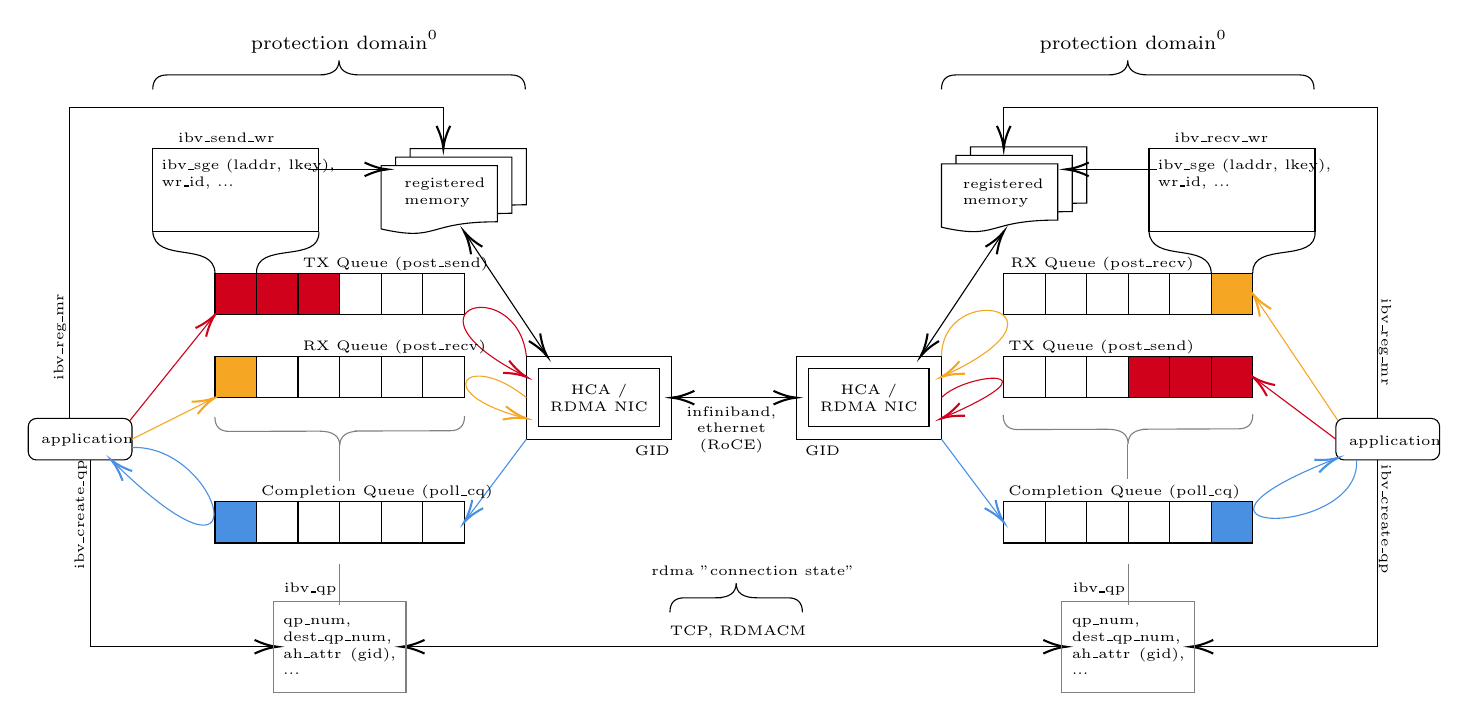
\begin{tikzpicture}[x=0.75pt,y=0.75pt,yscale=-1,xscale=1]
          \tikzset{every picture/.style={line width=0.75pt}} %set default line width to 0.75pt
%uncomment if require: \path (0,337); %set diagram left start at 0, and has height of 337

%Shape: Grid [id:dp4295659866532805]
\draw  [draw opacity=0] (100,220) -- (220,220) -- (220,240) -- (100,240) -- cycle ; \draw   (120,220) -- (120,240)(140,220) -- (140,240)(160,220) -- (160,240)(180,220) -- (180,240)(200,220) -- (200,240) ; \draw    ; \draw   (100,220) -- (220,220) -- (220,240) -- (100,240) -- cycle ;
%Shape: Grid [id:dp8946879606396433]
\draw  [draw opacity=0] (100,150) -- (220,150) -- (220,170) -- (100,170) -- cycle ; \draw   (120,150) -- (120,170)(140,150) -- (140,170)(160,150) -- (160,170)(180,150) -- (180,170)(200,150) -- (200,170) ; \draw    ; \draw   (100,150) -- (220,150) -- (220,170) -- (100,170) -- cycle ;
%Shape: Grid [id:dp4368011626744822]
\draw  [draw opacity=0] (100,110) -- (220,110) -- (220,130) -- (100,130) -- cycle ; \draw   (120,110) -- (120,130)(140,110) -- (140,130)(160,110) -- (160,130)(180,110) -- (180,130)(200,110) -- (200,130) ; \draw    ; \draw   (100,110) -- (220,110) -- (220,130) -- (100,130) -- cycle ;
%Shape: Frame [id:dp0617244658145758]
\draw   (250,150) -- (320,150) -- (320,190) -- (250,190) -- cycle(314,156) -- (256,156) -- (256,184) -- (314,184) -- cycle ;
%Curve Lines [id:da5967844605583035]
\draw [color={rgb, 255:red, 208; green, 2; blue, 27 }  ,draw opacity=1 ]   (250,150) .. controls (245.42,109.8) and (184.41,126.63) .. (249.02,159.5) ;
\draw [shift={(250,160)}, rotate = 206.63] [color={rgb, 255:red, 208; green, 2; blue, 27 }  ,draw opacity=1 ][line width=0.75]    (10.93,-3.29) .. controls (6.95,-1.4) and (3.31,-0.3) .. (0,0) .. controls (3.31,0.3) and (6.95,1.4) .. (10.93,3.29)   ;
%Straight Lines [id:da3545614732130127]
\draw [color={rgb, 255:red, 74; green, 144; blue, 226 }  ,draw opacity=1 ]   (250,190) -- (221.2,228.4) ;
\draw [shift={(220,230)}, rotate = 306.87] [color={rgb, 255:red, 74; green, 144; blue, 226 }  ,draw opacity=1 ][line width=0.75]    (10.93,-3.29) .. controls (6.95,-1.4) and (3.31,-0.3) .. (0,0) .. controls (3.31,0.3) and (6.95,1.4) .. (10.93,3.29)   ;
%Curve Lines [id:da204421881230066]
\draw [color={rgb, 255:red, 245; green, 166; blue, 35 }  ,draw opacity=1 ]   (250,170) .. controls (221.78,146.98) and (202.19,167.58) .. (248.57,179.64) ;
\draw [shift={(250,180)}, rotate = 193.98] [color={rgb, 255:red, 245; green, 166; blue, 35 }  ,draw opacity=1 ][line width=0.75]    (10.93,-3.29) .. controls (6.95,-1.4) and (3.31,-0.3) .. (0,0) .. controls (3.31,0.3) and (6.95,1.4) .. (10.93,3.29)   ;
%Shape: Rectangle [id:dp7444892557504112]
\draw   (70,50) -- (150,50) -- (150,90) -- (70,90) -- cycle ;
%Curve Lines [id:da4358799403511109]
\draw    (100,110) .. controls (99.4,94.4) and (71,105.6) .. (70,90) ;
%Curve Lines [id:da04054970173393413]
\draw    (120,110) .. controls (119.4,94.4) and (151,105.6) .. (150,90) ;
%Shape: Rectangle [id:dp09447409855918232]
\draw  [fill={rgb, 255:red, 208; green, 2; blue, 27 }  ,fill opacity=1 ] (140,110) -- (160,110) -- (160,130) -- (140,130) -- cycle ;
%Shape: Rectangle [id:dp7954961531438973]
\draw  [fill={rgb, 255:red, 208; green, 2; blue, 27 }  ,fill opacity=1 ] (120,110) -- (140,110) -- (140,130) -- (120,130) -- cycle ;
%Shape: Rectangle [id:dp375729093280755]
\draw  [fill={rgb, 255:red, 245; green, 166; blue, 35 }  ,fill opacity=1 ] (100,150) -- (120,150) -- (120,170) -- (100,170) -- cycle ;
%Shape: Rectangle [id:dp7009688837706805]
\draw  [fill={rgb, 255:red, 208; green, 2; blue, 27 }  ,fill opacity=1 ] (100,110) -- (120,110) -- (120,130) -- (100,130) -- cycle ;
%Shape: Rectangle [id:dp4753240489158659]
\draw  [fill={rgb, 255:red, 74; green, 144; blue, 226 }  ,fill opacity=1 ] (100,220) -- (120,220) -- (120,240) -- (100,240) -- cycle ;
%Rounded Rect [id:dp7482108927478565]
\draw   (10,184) .. controls (10,181.79) and (11.79,180) .. (14,180) -- (56,180) .. controls (58.21,180) and (60,181.79) .. (60,184) -- (60,196) .. controls (60,198.21) and (58.21,200) .. (56,200) -- (14,200) .. controls (11.79,200) and (10,198.21) .. (10,196) -- cycle ;
%Straight Lines [id:da0860623165459462]
\draw [color={rgb, 255:red, 208; green, 2; blue, 27 }  ,draw opacity=1 ]   (59,181) -- (98.75,131.56) ;
\draw [shift={(100,130)}, rotate = 488.8] [color={rgb, 255:red, 208; green, 2; blue, 27 }  ,draw opacity=1 ][line width=0.75]    (10.93,-3.29) .. controls (6.95,-1.4) and (3.31,-0.3) .. (0,0) .. controls (3.31,0.3) and (6.95,1.4) .. (10.93,3.29)   ;
%Straight Lines [id:da10819672911414313]
\draw [color={rgb, 255:red, 245; green, 166; blue, 35 }  ,draw opacity=1 ]   (60,190) -- (98.21,170.89) ;
\draw [shift={(100,170)}, rotate = 513.4300000000001] [color={rgb, 255:red, 245; green, 166; blue, 35 }  ,draw opacity=1 ][line width=0.75]    (10.93,-3.29) .. controls (6.95,-1.4) and (3.31,-0.3) .. (0,0) .. controls (3.31,0.3) and (6.95,1.4) .. (10.93,3.29)   ;
%Curve Lines [id:da5396028508269919]
\draw [color={rgb, 255:red, 74; green, 144; blue, 226 }  ,draw opacity=1 ]   (60,194) .. controls (102.79,192.41) and (125.18,273.98) .. (51.12,201.11) ;
\draw [shift={(50,200)}, rotate = 404.77] [color={rgb, 255:red, 74; green, 144; blue, 226 }  ,draw opacity=1 ][line width=0.75]    (10.93,-3.29) .. controls (6.95,-1.4) and (3.31,-0.3) .. (0,0) .. controls (3.31,0.3) and (6.95,1.4) .. (10.93,3.29)   ;
%Flowchart: Multidocument [id:dp5721236644573098]
\draw  [fill={rgb, 255:red, 255; green, 255; blue, 255 }  ,fill opacity=1 ] (194,50) -- (250,50) -- (250,77.06) .. controls (215,77.06) and (222,86.82) .. (194,80.5) -- cycle ; \draw  [fill={rgb, 255:red, 255; green, 255; blue, 255 }  ,fill opacity=1 ] (187,54.1) -- (243,54.1) -- (243,81.16) .. controls (208,81.16) and (215,90.92) .. (187,84.6) -- cycle ; \draw  [fill={rgb, 255:red, 255; green, 255; blue, 255 }  ,fill opacity=1 ] (180,58.2) -- (236,58.2) -- (236,85.26) .. controls (201,85.26) and (208,95.02) .. (180,88.7) -- cycle ;
%Straight Lines [id:da6912345896218269]
\draw    (145,60) -- (181,60) ;
\draw [shift={(183,60)}, rotate = 180] [color={rgb, 255:red, 0; green, 0; blue, 0 }  ][line width=0.75]    (10.93,-3.29) .. controls (6.95,-1.4) and (3.31,-0.3) .. (0,0) .. controls (3.31,0.3) and (6.95,1.4) .. (10.93,3.29)   ;
%Shape: Grid [id:dp119026641862925]
\draw  [draw opacity=0] (480,220) -- (600,220) -- (600,240) -- (480,240) -- cycle ; \draw   (500,220) -- (500,240)(520,220) -- (520,240)(540,220) -- (540,240)(560,220) -- (560,240)(580,220) -- (580,240) ; \draw    ; \draw   (480,220) -- (600,220) -- (600,240) -- (480,240) -- cycle ;
%Shape: Grid [id:dp0804991380561264]
\draw  [draw opacity=0] (480,150) -- (600,150) -- (600,170) -- (480,170) -- cycle ; \draw   (500,150) -- (500,170)(520,150) -- (520,170)(540,150) -- (540,170)(560,150) -- (560,170)(580,150) -- (580,170) ; \draw    ; \draw   (480,150) -- (600,150) -- (600,170) -- (480,170) -- cycle ;
%Shape: Grid [id:dp11715394785996025]
\draw  [draw opacity=0] (480,110) -- (600,110) -- (600,130) -- (480,130) -- cycle ; \draw   (500,110) -- (500,130)(520,110) -- (520,130)(540,110) -- (540,130)(560,110) -- (560,130)(580,110) -- (580,130) ; \draw    ; \draw   (480,110) -- (600,110) -- (600,130) -- (480,130) -- cycle ;
%Shape: Frame [id:dp8132523520793834]
\draw   (380,150) -- (450,150) -- (450,190) -- (380,190) -- cycle(444,156) -- (386,156) -- (386,184) -- (444,184) -- cycle ;
%Shape: Rectangle [id:dp9806953964426239]
\draw   (549.98,50) -- (629.98,50) -- (629.98,90) -- (549.98,90) -- cycle ;
%Curve Lines [id:da8538159727708337]
\draw    (579.98,110) .. controls (579.38,94.4) and (550.98,105.6) .. (549.98,90) ;
%Curve Lines [id:da503262725402064]
\draw    (599.98,110) .. controls (599.38,94.4) and (630.98,105.6) .. (629.98,90) ;
%Shape: Rectangle [id:dp23358801131092133]
\draw  [fill={rgb, 255:red, 208; green, 2; blue, 27 }  ,fill opacity=1 ] (580,150) -- (600,150) -- (600,170) -- (580,170) -- cycle ;
%Shape: Rectangle [id:dp16921311873779]
\draw  [fill={rgb, 255:red, 208; green, 2; blue, 27 }  ,fill opacity=1 ] (560,150) -- (580,150) -- (580,170) -- (560,170) -- cycle ;
%Shape: Rectangle [id:dp1685110147344583]
\draw  [fill={rgb, 255:red, 245; green, 166; blue, 35 }  ,fill opacity=1 ] (580,110) -- (600,110) -- (600,130) -- (580,130) -- cycle ;
%Shape: Rectangle [id:dp5932409601304787]
\draw  [fill={rgb, 255:red, 208; green, 2; blue, 27 }  ,fill opacity=1 ] (540,150) -- (560,150) -- (560,170) -- (540,170) -- cycle ;
%Shape: Rectangle [id:dp5864080847756401]
\draw  [fill={rgb, 255:red, 74; green, 144; blue, 226 }  ,fill opacity=1 ] (580,220) -- (600,220) -- (600,240) -- (580,240) -- cycle ;
%Rounded Rect [id:dp9740510619526319]
\draw   (640,184) .. controls (640,181.79) and (641.79,180) .. (644,180) -- (686,180) .. controls (688.21,180) and (690,181.79) .. (690,184) -- (690,196) .. controls (690,198.21) and (688.21,200) .. (686,200) -- (644,200) .. controls (641.79,200) and (640,198.21) .. (640,196) -- cycle ;
%Straight Lines [id:da16241601875679856]
\draw [color={rgb, 255:red, 208; green, 2; blue, 27 }  ,draw opacity=1 ]   (640,190) -- (601.6,161.2) ;
\draw [shift={(600,160)}, rotate = 396.87] [color={rgb, 255:red, 208; green, 2; blue, 27 }  ,draw opacity=1 ][line width=0.75]    (10.93,-3.29) .. controls (6.95,-1.4) and (3.31,-0.3) .. (0,0) .. controls (3.31,0.3) and (6.95,1.4) .. (10.93,3.29)   ;
%Straight Lines [id:da918563124412445]
\draw [color={rgb, 255:red, 245; green, 166; blue, 35 }  ,draw opacity=1 ]   (641,181) -- (601.12,121.66) ;
\draw [shift={(600,120)}, rotate = 416.09000000000003] [color={rgb, 255:red, 245; green, 166; blue, 35 }  ,draw opacity=1 ][line width=0.75]    (10.93,-3.29) .. controls (6.95,-1.4) and (3.31,-0.3) .. (0,0) .. controls (3.31,0.3) and (6.95,1.4) .. (10.93,3.29)   ;
%Curve Lines [id:da07688196394851687]
\draw [color={rgb, 255:red, 74; green, 144; blue, 226 }  ,draw opacity=1 ]   (650,200) .. controls (652.32,238.47) and (544.75,236.69) .. (639.56,199.56) ;
\draw [shift={(641,199)}, rotate = 518.8399999999999] [color={rgb, 255:red, 74; green, 144; blue, 226 }  ,draw opacity=1 ][line width=0.75]    (10.93,-3.29) .. controls (6.95,-1.4) and (3.31,-0.3) .. (0,0) .. controls (3.31,0.3) and (6.95,1.4) .. (10.93,3.29)   ;
%Flowchart: Multidocument [id:dp24323844239769876]
\draw  [fill={rgb, 255:red, 255; green, 255; blue, 255 }  ,fill opacity=1 ] (464,49.17) -- (520,49.17) -- (520,76.23) .. controls (485,76.23) and (492,85.99) .. (464,79.67) -- cycle ; \draw  [fill={rgb, 255:red, 255; green, 255; blue, 255 }  ,fill opacity=1 ] (457,53.27) -- (513,53.27) -- (513,80.33) .. controls (478,80.33) and (485,90.09) .. (457,83.77) -- cycle ; \draw  [fill={rgb, 255:red, 255; green, 255; blue, 255 }  ,fill opacity=1 ] (450,57.37) -- (506,57.37) -- (506,84.43) .. controls (471,84.43) and (478,94.19) .. (450,87.87) -- cycle ;
%Straight Lines [id:da7059822979397073]
\draw    (660,180) -- (660,30) ;
%Straight Lines [id:da481201579183531]
\draw    (512,60) -- (554,60) ;
\draw [shift={(510,60)}, rotate = 0] [color={rgb, 255:red, 0; green, 0; blue, 0 }  ][line width=0.75]    (10.93,-3.29) .. controls (6.95,-1.4) and (3.31,-0.3) .. (0,0) .. controls (3.31,0.3) and (6.95,1.4) .. (10.93,3.29)   ;
%Straight Lines [id:da22589634957435445]
\draw [color={rgb, 255:red, 0; green, 0; blue, 0 }  ,draw opacity=1 ]   (322,170) -- (378,170) ;
\draw [shift={(380,170)}, rotate = 180] [color={rgb, 255:red, 0; green, 0; blue, 0 }  ,draw opacity=1 ][line width=0.75]    (10.93,-3.29) .. controls (6.95,-1.4) and (3.31,-0.3) .. (0,0) .. controls (3.31,0.3) and (6.95,1.4) .. (10.93,3.29)   ;
\draw [shift={(320,170)}, rotate = 0] [color={rgb, 255:red, 0; green, 0; blue, 0 }  ,draw opacity=1 ][line width=0.75]    (10.93,-3.29) .. controls (6.95,-1.4) and (3.31,-0.3) .. (0,0) .. controls (3.31,0.3) and (6.95,1.4) .. (10.93,3.29)   ;
%Straight Lines [id:da11720587390108372]
\draw    (192,290) -- (508,290) ;
\draw [shift={(510,290)}, rotate = 180] [color={rgb, 255:red, 0; green, 0; blue, 0 }  ][line width=0.75]    (10.93,-3.29) .. controls (6.95,-1.4) and (3.31,-0.3) .. (0,0) .. controls (3.31,0.3) and (6.95,1.4) .. (10.93,3.29)   ;
\draw [shift={(190,290)}, rotate = 0] [color={rgb, 255:red, 0; green, 0; blue, 0 }  ][line width=0.75]    (10.93,-3.29) .. controls (6.95,-1.4) and (3.31,-0.3) .. (0,0) .. controls (3.31,0.3) and (6.95,1.4) .. (10.93,3.29)   ;
%Curve Lines [id:da21032506501189785]
\draw [color={rgb, 255:red, 245; green, 166; blue, 35 }  ,draw opacity=1 ]   (450,150) .. controls (450.6,112.59) and (520.69,127.45) .. (451.06,159.52) ;
\draw [shift={(450,160)}, rotate = 335.59000000000003] [color={rgb, 255:red, 245; green, 166; blue, 35 }  ,draw opacity=1 ][line width=0.75]    (10.93,-3.29) .. controls (6.95,-1.4) and (3.31,-0.3) .. (0,0) .. controls (3.31,0.3) and (6.95,1.4) .. (10.93,3.29)   ;
%Curve Lines [id:da1795237296648432]
\draw [color={rgb, 255:red, 208; green, 2; blue, 27 }  ,draw opacity=1 ]   (450,170) .. controls (461.68,157.72) and (508.84,154.46) .. (451.76,179.24) ;
\draw [shift={(450,180)}, rotate = 336.82] [color={rgb, 255:red, 208; green, 2; blue, 27 }  ,draw opacity=1 ][line width=0.75]    (10.93,-3.29) .. controls (6.95,-1.4) and (3.31,-0.3) .. (0,0) .. controls (3.31,0.3) and (6.95,1.4) .. (10.93,3.29)   ;
%Straight Lines [id:da2007010103317477]
\draw [color={rgb, 255:red, 74; green, 144; blue, 226 }  ,draw opacity=1 ]   (450,190) -- (478.8,228.4) ;
\draw [shift={(480,230)}, rotate = 233.13] [color={rgb, 255:red, 74; green, 144; blue, 226 }  ,draw opacity=1 ][line width=0.75]    (10.93,-3.29) .. controls (6.95,-1.4) and (3.31,-0.3) .. (0,0) .. controls (3.31,0.3) and (6.95,1.4) .. (10.93,3.29)   ;
%Shape: Brace [id:dp9940577590245101]
\draw   (383,273.42) .. controls (383,268.75) and (380.67,266.42) .. (376,266.42) -- (361.08,266.42) .. controls (354.41,266.42) and (351.08,264.09) .. (351.08,259.42) .. controls (351.08,264.09) and (347.75,266.42) .. (341.08,266.42)(344.08,266.42) -- (326.17,266.42) .. controls (321.5,266.42) and (319.17,268.75) .. (319.17,273.42) ;
%Straight Lines [id:da4361920428251189]
\draw    (660,200) -- (660,290) ;
%Straight Lines [id:da480314407062288]
\draw    (40,200) -- (40,290) ;
%Shape: Brace [id:dp588298908527398]
\draw  [color={rgb, 255:red, 128; green, 128; blue, 128 }  ,draw opacity=1 ] (99.93,179.28) .. controls (99.95,183.95) and (102.29,186.27) .. (106.96,186.26) -- (150.09,186.13) .. controls (156.76,186.1) and (160.1,188.42) .. (160.11,193.09) .. controls (160.1,188.42) and (163.42,186.08) .. (170.09,186.06)(167.09,186.07) -- (213.22,185.93) .. controls (217.89,185.92) and (220.21,183.58) .. (220.2,178.91) ;
%Straight Lines [id:da0889380362629657]
\draw    (40,290) -- (128,290) ;
\draw [shift={(130,290)}, rotate = 180] [color={rgb, 255:red, 0; green, 0; blue, 0 }  ][line width=0.75]    (10.93,-3.29) .. controls (6.95,-1.4) and (3.31,-0.3) .. (0,0) .. controls (3.31,0.3) and (6.95,1.4) .. (10.93,3.29)   ;
%Straight Lines [id:da17063350648323872]
\draw [color={rgb, 255:red, 128; green, 128; blue, 128 }  ,draw opacity=1 ]   (160,193) -- (160,210) ;
%Straight Lines [id:da735591769614332]
\draw [color={rgb, 255:red, 128; green, 128; blue, 128 }  ,draw opacity=1 ]   (160,250) -- (160,270) ;
%Shape: Brace [id:dp7463787220884971]
\draw  [color={rgb, 255:red, 128; green, 128; blue, 128 }  ,draw opacity=1 ] (479.73,178.38) .. controls (479.75,183.05) and (482.09,185.37) .. (486.76,185.36) -- (529.89,185.22) .. controls (536.56,185.2) and (539.9,187.52) .. (539.91,192.19) .. controls (539.9,187.52) and (543.22,185.18) .. (549.89,185.16)(546.89,185.17) -- (593.02,185.02) .. controls (597.69,185.01) and (600.01,182.67) .. (600,178) ;
%Straight Lines [id:da6347067855883498]
\draw [color={rgb, 255:red, 128; green, 128; blue, 128 }  ,draw opacity=1 ]   (539.8,192.09) -- (539.8,209.09) ;
%Straight Lines [id:da7879312663238379]
\draw [color={rgb, 255:red, 128; green, 128; blue, 128 }  ,draw opacity=1 ]   (540,250) -- (540,270) ;
%Straight Lines [id:da34735570105619973]
\draw    (660,290) -- (572,290) ;
\draw [shift={(570,290)}, rotate = 360] [color={rgb, 255:red, 0; green, 0; blue, 0 }  ][line width=0.75]    (10.93,-3.29) .. controls (6.95,-1.4) and (3.31,-0.3) .. (0,0) .. controls (3.31,0.3) and (6.95,1.4) .. (10.93,3.29)   ;
%Straight Lines [id:da6922947722733842]
\draw    (480,30) -- (660,30) ;
%Straight Lines [id:da8214317936198106]
\draw    (480,30) -- (480,48) ;
\draw [shift={(480,50)}, rotate = 270] [color={rgb, 255:red, 0; green, 0; blue, 0 }  ][line width=0.75]    (10.93,-3.29) .. controls (6.95,-1.4) and (3.31,-0.3) .. (0,0) .. controls (3.31,0.3) and (6.95,1.4) .. (10.93,3.29)   ;
%Straight Lines [id:da3127224438135543]
\draw    (30,180) -- (30,30) ;
%Straight Lines [id:da25223149816814294]
\draw    (30,30) -- (210,30) ;
%Straight Lines [id:da6150923577431217]
\draw    (210,30) -- (210,48) ;
\draw [shift={(210,50)}, rotate = 270] [color={rgb, 255:red, 0; green, 0; blue, 0 }  ][line width=0.75]    (10.93,-3.29) .. controls (6.95,-1.4) and (3.31,-0.3) .. (0,0) .. controls (3.31,0.3) and (6.95,1.4) .. (10.93,3.29)   ;
%Shape: Brace [id:dp7460733200764286]
\draw   (249.5,21.5) .. controls (249.5,16.83) and (247.17,14.5) .. (242.5,14.5) -- (169.75,14.5) .. controls (163.08,14.5) and (159.75,12.17) .. (159.75,7.5) .. controls (159.75,12.17) and (156.42,14.5) .. (149.75,14.5)(152.75,14.5) -- (77,14.5) .. controls (72.33,14.5) and (70,16.83) .. (70,21.5) ;
%Shape: Brace [id:dp25327117875899263]
\draw   (629.5,21.5) .. controls (629.5,16.83) and (627.17,14.5) .. (622.5,14.5) -- (549.75,14.5) .. controls (543.08,14.5) and (539.75,12.17) .. (539.75,7.5) .. controls (539.75,12.17) and (536.42,14.5) .. (529.75,14.5)(532.75,14.5) -- (457,14.5) .. controls (452.33,14.5) and (450,16.83) .. (450,21.5) ;
%Straight Lines [id:da5693657957631059]
\draw    (221.11,91.66) -- (258.89,148.34) ;
\draw [shift={(260,150)}, rotate = 236.31] [color={rgb, 255:red, 0; green, 0; blue, 0 }  ][line width=0.75]    (10.93,-3.29) .. controls (6.95,-1.4) and (3.31,-0.3) .. (0,0) .. controls (3.31,0.3) and (6.95,1.4) .. (10.93,3.29)   ;
\draw [shift={(220,90)}, rotate = 56.31] [color={rgb, 255:red, 0; green, 0; blue, 0 }  ][line width=0.75]    (10.93,-3.29) .. controls (6.95,-1.4) and (3.31,-0.3) .. (0,0) .. controls (3.31,0.3) and (6.95,1.4) .. (10.93,3.29)   ;
%Straight Lines [id:da648148726214795]
\draw    (478.89,91.66) -- (441.11,148.34) ;
\draw [shift={(440,150)}, rotate = 303.69] [color={rgb, 255:red, 0; green, 0; blue, 0 }  ][line width=0.75]    (10.93,-3.29) .. controls (6.95,-1.4) and (3.31,-0.3) .. (0,0) .. controls (3.31,0.3) and (6.95,1.4) .. (10.93,3.29)   ;
\draw [shift={(480,90)}, rotate = 123.69] [color={rgb, 255:red, 0; green, 0; blue, 0 }  ][line width=0.75]    (10.93,-3.29) .. controls (6.95,-1.4) and (3.31,-0.3) .. (0,0) .. controls (3.31,0.3) and (6.95,1.4) .. (10.93,3.29)   ;

% Text Node
\draw (121,211) node [anchor=north west][inner sep=0.75pt]  [font=\tiny] [align=left] {Completion Queue (poll\_cq)};
% Text Node
\draw (141,101) node [anchor=north west][inner sep=0.75pt]  [font=\tiny] [align=left] {TX Queue (post\_send)};
% Text Node
\draw (141,141) node [anchor=north west][inner sep=0.75pt]  [font=\tiny] [align=left] {RX Queue (post\_recv)};
% Text Node
\draw (81,41) node [anchor=north west][inner sep=0.75pt]  [font=\tiny] [align=left] {ibv\_send\_wr};
% Text Node
\draw (73,54) node [anchor=north west][inner sep=0.75pt]  [font=\tiny] [align=left] {ibv\_sge (laddr, lkey),\\wr\_id, ...};
% Text Node
\draw (15,186) node [anchor=north west][inner sep=0.75pt]  [font=\tiny] [align=left] {application};
% Text Node
\draw (190,63) node [anchor=north west][inner sep=0.75pt]  [font=\tiny] [align=left] {registered\\memory};
% Text Node
\draw (21,163) node [anchor=north west][inner sep=0.75pt]  [font=\tiny,rotate=-270] [align=left] {ibv\_reg\_mr};
% Text Node
\draw (481,141) node [anchor=north west][inner sep=0.75pt]  [font=\tiny] [align=left] {TX Queue (post\_send)};
% Text Node
\draw (482,101) node [anchor=north west][inner sep=0.75pt]  [font=\tiny] [align=left] {RX Queue (post\_recv)};
% Text Node
\draw (560.98,41) node [anchor=north west][inner sep=0.75pt]  [font=\tiny] [align=left] {ibv\_recv\_wr};
% Text Node
\draw (552.98,54) node [anchor=north west][inner sep=0.75pt]  [font=\tiny] [align=left] {ibv\_sge (laddr, lkey),\\wr\_id, ...};
% Text Node
\draw (645,187) node [anchor=north west][inner sep=0.75pt]  [font=\tiny] [align=left] {application};
% Text Node
\draw (459,63.17) node [anchor=north west][inner sep=0.75pt]  [font=\tiny] [align=left] {registered\\memory};
% Text Node
\draw (668,121) node [anchor=north west][inner sep=0.75pt]  [font=\tiny,rotate=-90] [align=left] {ibv\_reg\_mr};
% Text Node
\draw (321,173) node [anchor=north west][inner sep=0.75pt]  [font=\tiny] [align=left] {\begin{minipage}[lt]{39.83664400000001pt}\setlength\topsep{0pt}
\begin{center}
infiniband,\\ethernet (RoCE)
\end{center}

\end{minipage}};
% Text Node
\draw (481,211) node [anchor=north west][inner sep=0.75pt]  [font=\tiny] [align=left] {Completion Queue (poll\_cq)};
% Text Node
\draw (285,170) node  [font=\tiny] [align=left] {\begin{minipage}[lt]{39.440000000000005pt}\setlength\topsep{0pt}
\begin{center}
HCA /\\RDMA NIC
\end{center}

\end{minipage}};
% Text Node
\draw (415,170) node  [font=\tiny] [align=left] {\begin{minipage}[lt]{39.440000000000005pt}\setlength\topsep{0pt}
\begin{center}
HCA /\\RDMA NIC
\end{center}

\end{minipage}};
% Text Node
\draw (301,192) node [anchor=north west][inner sep=0.75pt]  [font=\tiny] [align=left] {GID};
% Text Node
\draw (383,192) node [anchor=north west][inner sep=0.75pt]  [font=\tiny] [align=left] {GID};
% Text Node
\draw  [color={rgb, 255:red, 128; green, 128; blue, 128 }  ,draw opacity=1 ]  (128,268) -- (192,268) -- (192,312) -- (128,312) -- cycle  ;
\draw (160,290) node  [font=\tiny] [align=left] {\begin{minipage}[lt]{40.800000000000004pt}\setlength\topsep{0pt}
qp\_num, dest\_qp\_num, ah\_attr (gid), ...
\end{minipage}};
% Text Node
\draw (132,258) node [anchor=north west][inner sep=0.75pt]  [font=\tiny] [align=left] {ibv\_qp};
% Text Node
\draw (309,250) node [anchor=north west][inner sep=0.75pt]  [font=\tiny] [align=left] {rdma "connection state"};
% Text Node
\draw (31,254) node [anchor=north west][inner sep=0.75pt]  [font=\tiny,rotate=-270] [align=left] {ibv\_create\_qp};
% Text Node
\draw (668,201) node [anchor=north west][inner sep=0.75pt]  [font=\tiny,rotate=-90] [align=left] {ibv\_create\_qp};
% Text Node
\draw (352,283) node  [font=\tiny] [align=left] {\begin{minipage}[lt]{68pt}\setlength\topsep{0pt}
\begin{center}
TCP, RDMACM
\end{center}

\end{minipage}};
% Text Node
\draw  [color={rgb, 255:red, 128; green, 128; blue, 128 }  ,draw opacity=1 ]  (508,268) -- (572,268) -- (572,312) -- (508,312) -- cycle  ;
\draw (540,290) node  [font=\tiny] [align=left] {\begin{minipage}[lt]{40.800000000000004pt}\setlength\topsep{0pt}
qp\_num, dest\_qp\_num, ah\_attr (gid), ...
\end{minipage}};
% Text Node
\draw (512,258) node [anchor=north west][inner sep=0.75pt]  [font=\tiny] [align=left] {ibv\_qp};
% Text Node
\draw (116,-8) node [anchor=north west][inner sep=0.75pt]  [font=\scriptsize] [align=left] {protection domain$\displaystyle ^{0}$};
% Text Node
\draw (496,-8) node [anchor=north west][inner sep=0.75pt]  [font=\scriptsize] [align=left] {protection domain$\displaystyle ^{0}$};

      \end{tikzpicture}
  }
  \footnotetext{\tiny Every object in the protection domain is mapped in the application's virtual address space. The HCA can access every object in the protection domain.}
\end{frame}

\begin{frame}[fragile]{RDMA One-Sided Ops}
  \resizebox{\textwidth}{!}{
      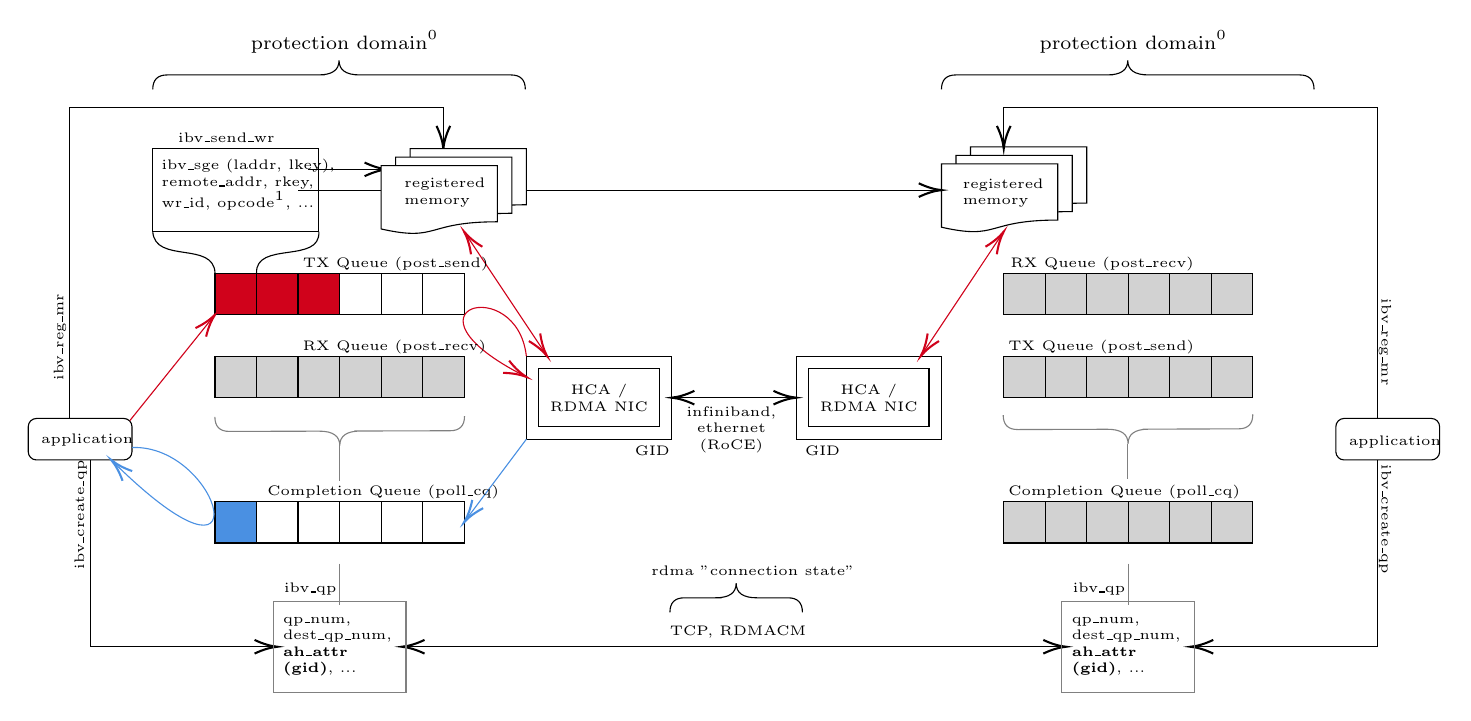
\begin{tikzpicture}[x=0.75pt,y=0.75pt,yscale=-1,xscale=1]
          \tikzset{every picture/.style={line width=0.75pt}} %set default line width to 0.75pt
%uncomment if require: \path (0,337); %set diagram left start at 0, and has height of 337

%Shape: Grid [id:dp3947000390218536]
\draw  [draw opacity=0] (100,220) -- (220,220) -- (220,240) -- (100,240) -- cycle ; \draw   (120,220) -- (120,240)(140,220) -- (140,240)(160,220) -- (160,240)(180,220) -- (180,240)(200,220) -- (200,240) ; \draw    ; \draw   (100,220) -- (220,220) -- (220,240) -- (100,240) -- cycle ;
%Shape: Grid [id:dp22641340768149854]
\draw  [draw opacity=0][fill={rgb, 255:red, 210; green, 210; blue, 210 }  ,fill opacity=1 ] (100,150) -- (220,150) -- (220,170) -- (100,170) -- cycle ; \draw   (120,150) -- (120,170)(140,150) -- (140,170)(160,150) -- (160,170)(180,150) -- (180,170)(200,150) -- (200,170) ; \draw    ; \draw   (100,150) -- (220,150) -- (220,170) -- (100,170) -- cycle ;
%Shape: Grid [id:dp4235937886523329]
\draw  [draw opacity=0] (100,110) -- (220,110) -- (220,130) -- (100,130) -- cycle ; \draw   (120,110) -- (120,130)(140,110) -- (140,130)(160,110) -- (160,130)(180,110) -- (180,130)(200,110) -- (200,130) ; \draw    ; \draw   (100,110) -- (220,110) -- (220,130) -- (100,130) -- cycle ;
%Shape: Frame [id:dp012050559479128475]
\draw   (250,150) -- (320,150) -- (320,190) -- (250,190) -- cycle(314,156) -- (256,156) -- (256,184) -- (314,184) -- cycle ;
%Curve Lines [id:da31463783025150893]
\draw [color={rgb, 255:red, 208; green, 2; blue, 27 }  ,draw opacity=1 ]   (250,150) .. controls (245.42,109.8) and (184.41,126.63) .. (249.02,159.5) ;
\draw [shift={(250,160)}, rotate = 206.63] [color={rgb, 255:red, 208; green, 2; blue, 27 }  ,draw opacity=1 ][line width=0.75]    (10.93,-3.29) .. controls (6.95,-1.4) and (3.31,-0.3) .. (0,0) .. controls (3.31,0.3) and (6.95,1.4) .. (10.93,3.29)   ;
%Straight Lines [id:da7501929461239948]
\draw [color={rgb, 255:red, 74; green, 144; blue, 226 }  ,draw opacity=1 ]   (250,190) -- (221.2,228.4) ;
\draw [shift={(220,230)}, rotate = 306.87] [color={rgb, 255:red, 74; green, 144; blue, 226 }  ,draw opacity=1 ][line width=0.75]    (10.93,-3.29) .. controls (6.95,-1.4) and (3.31,-0.3) .. (0,0) .. controls (3.31,0.3) and (6.95,1.4) .. (10.93,3.29)   ;
%Shape: Rectangle [id:dp6807903002598301]
\draw   (70,50) -- (150,50) -- (150,90) -- (70,90) -- cycle ;
%Curve Lines [id:da35169652774060867]
\draw    (100,110) .. controls (99.4,94.4) and (71,105.6) .. (70,90) ;
%Curve Lines [id:da754076319081873]
\draw    (120,110) .. controls (119.4,94.4) and (151,105.6) .. (150,90) ;
%Shape: Rectangle [id:dp588441855959041]
\draw  [fill={rgb, 255:red, 208; green, 2; blue, 27 }  ,fill opacity=1 ] (140,110) -- (160,110) -- (160,130) -- (140,130) -- cycle ;
%Shape: Rectangle [id:dp057925550319075314]
\draw  [fill={rgb, 255:red, 208; green, 2; blue, 27 }  ,fill opacity=1 ] (120,110) -- (140,110) -- (140,130) -- (120,130) -- cycle ;
%Shape: Rectangle [id:dp12879856227198072]
\draw  [fill={rgb, 255:red, 208; green, 2; blue, 27 }  ,fill opacity=1 ] (100,110) -- (120,110) -- (120,130) -- (100,130) -- cycle ;
%Shape: Rectangle [id:dp8569540621368663]
\draw  [fill={rgb, 255:red, 74; green, 144; blue, 226 }  ,fill opacity=1 ] (100,220) -- (120,220) -- (120,240) -- (100,240) -- cycle ;
%Rounded Rect [id:dp3296638061414221]
\draw   (10,184) .. controls (10,181.79) and (11.79,180) .. (14,180) -- (56,180) .. controls (58.21,180) and (60,181.79) .. (60,184) -- (60,196) .. controls (60,198.21) and (58.21,200) .. (56,200) -- (14,200) .. controls (11.79,200) and (10,198.21) .. (10,196) -- cycle ;
%Straight Lines [id:da0573065923905397]
\draw [color={rgb, 255:red, 208; green, 2; blue, 27 }  ,draw opacity=1 ]   (59,181) -- (98.75,131.56) ;
\draw [shift={(100,130)}, rotate = 488.8] [color={rgb, 255:red, 208; green, 2; blue, 27 }  ,draw opacity=1 ][line width=0.75]    (10.93,-3.29) .. controls (6.95,-1.4) and (3.31,-0.3) .. (0,0) .. controls (3.31,0.3) and (6.95,1.4) .. (10.93,3.29)   ;
%Curve Lines [id:da9753037711052992]
\draw [color={rgb, 255:red, 74; green, 144; blue, 226 }  ,draw opacity=1 ]   (60,194) .. controls (102.79,192.41) and (125.18,273.98) .. (51.12,201.11) ;
\draw [shift={(50,200)}, rotate = 404.77] [color={rgb, 255:red, 74; green, 144; blue, 226 }  ,draw opacity=1 ][line width=0.75]    (10.93,-3.29) .. controls (6.95,-1.4) and (3.31,-0.3) .. (0,0) .. controls (3.31,0.3) and (6.95,1.4) .. (10.93,3.29)   ;
%Straight Lines [id:da1699512585602425]
\draw    (145,60) -- (181,60) ;
\draw [shift={(183,60)}, rotate = 180] [color={rgb, 255:red, 0; green, 0; blue, 0 }  ][line width=0.75]    (10.93,-3.29) .. controls (6.95,-1.4) and (3.31,-0.3) .. (0,0) .. controls (3.31,0.3) and (6.95,1.4) .. (10.93,3.29)   ;
%Shape: Grid [id:dp2428141205939126]
\draw  [draw opacity=0][fill={rgb, 255:red, 210; green, 210; blue, 210 }  ,fill opacity=1 ] (480,220) -- (600,220) -- (600,240) -- (480,240) -- cycle ; \draw   (500,220) -- (500,240)(520,220) -- (520,240)(540,220) -- (540,240)(560,220) -- (560,240)(580,220) -- (580,240) ; \draw    ; \draw   (480,220) -- (600,220) -- (600,240) -- (480,240) -- cycle ;
%Shape: Grid [id:dp5871287897247738]
\draw  [draw opacity=0][fill={rgb, 255:red, 210; green, 210; blue, 210 }  ,fill opacity=1 ] (480,150) -- (600,150) -- (600,170) -- (480,170) -- cycle ; \draw   (500,150) -- (500,170)(520,150) -- (520,170)(540,150) -- (540,170)(560,150) -- (560,170)(580,150) -- (580,170) ; \draw    ; \draw   (480,150) -- (600,150) -- (600,170) -- (480,170) -- cycle ;
%Shape: Grid [id:dp6666114464438736]
\draw  [draw opacity=0][fill={rgb, 255:red, 210; green, 210; blue, 210 }  ,fill opacity=1 ] (480,110) -- (600,110) -- (600,130) -- (480,130) -- cycle ; \draw   (500,110) -- (500,130)(520,110) -- (520,130)(540,110) -- (540,130)(560,110) -- (560,130)(580,110) -- (580,130) ; \draw    ; \draw   (480,110) -- (600,110) -- (600,130) -- (480,130) -- cycle ;
%Shape: Frame [id:dp33988465631687736]
\draw   (380,150) -- (450,150) -- (450,190) -- (380,190) -- cycle(444,156) -- (386,156) -- (386,184) -- (444,184) -- cycle ;
%Rounded Rect [id:dp9290011454602596]
\draw   (640,184) .. controls (640,181.79) and (641.79,180) .. (644,180) -- (686,180) .. controls (688.21,180) and (690,181.79) .. (690,184) -- (690,196) .. controls (690,198.21) and (688.21,200) .. (686,200) -- (644,200) .. controls (641.79,200) and (640,198.21) .. (640,196) -- cycle ;
%Flowchart: Multidocument [id:dp4109756106655085]
\draw  [fill={rgb, 255:red, 255; green, 255; blue, 255 }  ,fill opacity=1 ] (464,49.17) -- (520,49.17) -- (520,76.23) .. controls (485,76.23) and (492,85.99) .. (464,79.67) -- cycle ; \draw  [fill={rgb, 255:red, 255; green, 255; blue, 255 }  ,fill opacity=1 ] (457,53.27) -- (513,53.27) -- (513,80.33) .. controls (478,80.33) and (485,90.09) .. (457,83.77) -- cycle ; \draw  [fill={rgb, 255:red, 255; green, 255; blue, 255 }  ,fill opacity=1 ] (450,57.37) -- (506,57.37) -- (506,84.43) .. controls (471,84.43) and (478,94.19) .. (450,87.87) -- cycle ;
%Straight Lines [id:da1921302075296969]
\draw    (660,180) -- (660,30) ;
%Straight Lines [id:da37762407104575435]
\draw [color={rgb, 255:red, 0; green, 0; blue, 0 }  ,draw opacity=1 ]   (322,170) -- (378,170) ;
\draw [shift={(380,170)}, rotate = 180] [color={rgb, 255:red, 0; green, 0; blue, 0 }  ,draw opacity=1 ][line width=0.75]    (10.93,-3.29) .. controls (6.95,-1.4) and (3.31,-0.3) .. (0,0) .. controls (3.31,0.3) and (6.95,1.4) .. (10.93,3.29)   ;
\draw [shift={(320,170)}, rotate = 0] [color={rgb, 255:red, 0; green, 0; blue, 0 }  ,draw opacity=1 ][line width=0.75]    (10.93,-3.29) .. controls (6.95,-1.4) and (3.31,-0.3) .. (0,0) .. controls (3.31,0.3) and (6.95,1.4) .. (10.93,3.29)   ;
%Straight Lines [id:da5042379274745459]
\draw    (192,290) -- (508,290) ;
\draw [shift={(510,290)}, rotate = 180] [color={rgb, 255:red, 0; green, 0; blue, 0 }  ][line width=0.75]    (10.93,-3.29) .. controls (6.95,-1.4) and (3.31,-0.3) .. (0,0) .. controls (3.31,0.3) and (6.95,1.4) .. (10.93,3.29)   ;
\draw [shift={(190,290)}, rotate = 0] [color={rgb, 255:red, 0; green, 0; blue, 0 }  ][line width=0.75]    (10.93,-3.29) .. controls (6.95,-1.4) and (3.31,-0.3) .. (0,0) .. controls (3.31,0.3) and (6.95,1.4) .. (10.93,3.29)   ;
%Shape: Brace [id:dp13922096266535533]
\draw   (383,273.42) .. controls (383,268.75) and (380.67,266.42) .. (376,266.42) -- (361.08,266.42) .. controls (354.41,266.42) and (351.08,264.09) .. (351.08,259.42) .. controls (351.08,264.09) and (347.75,266.42) .. (341.08,266.42)(344.08,266.42) -- (326.17,266.42) .. controls (321.5,266.42) and (319.17,268.75) .. (319.17,273.42) ;
%Straight Lines [id:da16516725886398242]
\draw    (660,200) -- (660,290) ;
%Straight Lines [id:da10301010007850087]
\draw    (40,200) -- (40,290) ;
%Shape: Brace [id:dp3296890418112731]
\draw  [color={rgb, 255:red, 128; green, 128; blue, 128 }  ,draw opacity=1 ] (99.93,179.28) .. controls (99.95,183.95) and (102.29,186.27) .. (106.96,186.26) -- (150.09,186.13) .. controls (156.76,186.1) and (160.1,188.42) .. (160.11,193.09) .. controls (160.1,188.42) and (163.42,186.08) .. (170.09,186.06)(167.09,186.07) -- (213.22,185.93) .. controls (217.89,185.92) and (220.21,183.58) .. (220.2,178.91) ;
%Straight Lines [id:da9992434560656075]
\draw    (40,290) -- (128,290) ;
\draw [shift={(130,290)}, rotate = 180] [color={rgb, 255:red, 0; green, 0; blue, 0 }  ][line width=0.75]    (10.93,-3.29) .. controls (6.95,-1.4) and (3.31,-0.3) .. (0,0) .. controls (3.31,0.3) and (6.95,1.4) .. (10.93,3.29)   ;
%Straight Lines [id:da5342875036200526]
\draw [color={rgb, 255:red, 128; green, 128; blue, 128 }  ,draw opacity=1 ]   (160,193) -- (160,210) ;
%Straight Lines [id:da9339474764881227]
\draw [color={rgb, 255:red, 128; green, 128; blue, 128 }  ,draw opacity=1 ]   (160,250) -- (160,270) ;
%Shape: Brace [id:dp22093818384828245]
\draw  [color={rgb, 255:red, 128; green, 128; blue, 128 }  ,draw opacity=1 ] (479.73,178.38) .. controls (479.75,183.05) and (482.09,185.37) .. (486.76,185.36) -- (529.89,185.22) .. controls (536.56,185.2) and (539.9,187.52) .. (539.91,192.19) .. controls (539.9,187.52) and (543.22,185.18) .. (549.89,185.16)(546.89,185.17) -- (593.02,185.02) .. controls (597.69,185.01) and (600.01,182.67) .. (600,178) ;
%Straight Lines [id:da5623601074952965]
\draw [color={rgb, 255:red, 128; green, 128; blue, 128 }  ,draw opacity=1 ]   (539.8,192.09) -- (539.8,209.09) ;
%Straight Lines [id:da6337433675448425]
\draw [color={rgb, 255:red, 128; green, 128; blue, 128 }  ,draw opacity=1 ]   (540,250) -- (540,270) ;
%Straight Lines [id:da566906802253018]
\draw    (660,290) -- (572,290) ;
\draw [shift={(570,290)}, rotate = 360] [color={rgb, 255:red, 0; green, 0; blue, 0 }  ][line width=0.75]    (10.93,-3.29) .. controls (6.95,-1.4) and (3.31,-0.3) .. (0,0) .. controls (3.31,0.3) and (6.95,1.4) .. (10.93,3.29)   ;
%Straight Lines [id:da12493314116335974]
\draw    (480,30) -- (660,30) ;
%Straight Lines [id:da6073242584581408]
\draw    (480,30) -- (480,48) ;
\draw [shift={(480,50)}, rotate = 270] [color={rgb, 255:red, 0; green, 0; blue, 0 }  ][line width=0.75]    (10.93,-3.29) .. controls (6.95,-1.4) and (3.31,-0.3) .. (0,0) .. controls (3.31,0.3) and (6.95,1.4) .. (10.93,3.29)   ;
%Straight Lines [id:da6124365265915639]
\draw    (30,180) -- (30,30) ;
%Straight Lines [id:da12995738416833458]
\draw    (30,30) -- (210,30) ;
%Straight Lines [id:da5704905331278706]
\draw    (210,30) -- (210,48) ;
\draw [shift={(210,50)}, rotate = 270] [color={rgb, 255:red, 0; green, 0; blue, 0 }  ][line width=0.75]    (10.93,-3.29) .. controls (6.95,-1.4) and (3.31,-0.3) .. (0,0) .. controls (3.31,0.3) and (6.95,1.4) .. (10.93,3.29)   ;
%Shape: Brace [id:dp9159228067295668]
\draw   (249.5,21.5) .. controls (249.5,16.83) and (247.17,14.5) .. (242.5,14.5) -- (169.75,14.5) .. controls (163.08,14.5) and (159.75,12.17) .. (159.75,7.5) .. controls (159.75,12.17) and (156.42,14.5) .. (149.75,14.5)(152.75,14.5) -- (77,14.5) .. controls (72.33,14.5) and (70,16.83) .. (70,21.5) ;
%Shape: Brace [id:dp7907821455624611]
\draw   (629.5,21.5) .. controls (629.5,16.83) and (627.17,14.5) .. (622.5,14.5) -- (549.75,14.5) .. controls (543.08,14.5) and (539.75,12.17) .. (539.75,7.5) .. controls (539.75,12.17) and (536.42,14.5) .. (529.75,14.5)(532.75,14.5) -- (457,14.5) .. controls (452.33,14.5) and (450,16.83) .. (450,21.5) ;
%Straight Lines [id:da5047287481524281]
\draw [color={rgb, 255:red, 208; green, 2; blue, 27 }  ,draw opacity=1 ]   (221.11,91.66) -- (258.89,148.34) ;
\draw [shift={(260,150)}, rotate = 236.31] [color={rgb, 255:red, 208; green, 2; blue, 27 }  ,draw opacity=1 ][line width=0.75]    (10.93,-3.29) .. controls (6.95,-1.4) and (3.31,-0.3) .. (0,0) .. controls (3.31,0.3) and (6.95,1.4) .. (10.93,3.29)   ;
\draw [shift={(220,90)}, rotate = 56.31] [color={rgb, 255:red, 208; green, 2; blue, 27 }  ,draw opacity=1 ][line width=0.75]    (10.93,-3.29) .. controls (6.95,-1.4) and (3.31,-0.3) .. (0,0) .. controls (3.31,0.3) and (6.95,1.4) .. (10.93,3.29)   ;
%Straight Lines [id:da2701646088561559]
\draw [color={rgb, 255:red, 208; green, 2; blue, 27 }  ,draw opacity=1 ]   (478.89,91.66) -- (441.11,148.34) ;
\draw [shift={(440,150)}, rotate = 303.69] [color={rgb, 255:red, 208; green, 2; blue, 27 }  ,draw opacity=1 ][line width=0.75]    (10.93,-3.29) .. controls (6.95,-1.4) and (3.31,-0.3) .. (0,0) .. controls (3.31,0.3) and (6.95,1.4) .. (10.93,3.29)   ;
\draw [shift={(480,90)}, rotate = 123.69] [color={rgb, 255:red, 208; green, 2; blue, 27 }  ,draw opacity=1 ][line width=0.75]    (10.93,-3.29) .. controls (6.95,-1.4) and (3.31,-0.3) .. (0,0) .. controls (3.31,0.3) and (6.95,1.4) .. (10.93,3.29)   ;
%Straight Lines [id:da8965354386782155]
\draw    (140,70) -- (448,70) ;
\draw [shift={(450,70)}, rotate = 180] [color={rgb, 255:red, 0; green, 0; blue, 0 }  ][line width=0.75]    (10.93,-3.29) .. controls (6.95,-1.4) and (3.31,-0.3) .. (0,0) .. controls (3.31,0.3) and (6.95,1.4) .. (10.93,3.29)   ;
%Flowchart: Multidocument [id:dp1393375731541463]
\draw  [fill={rgb, 255:red, 255; green, 255; blue, 255 }  ,fill opacity=1 ] (194,50) -- (250,50) -- (250,77.06) .. controls (215,77.06) and (222,86.82) .. (194,80.5) -- cycle ; \draw  [fill={rgb, 255:red, 255; green, 255; blue, 255 }  ,fill opacity=1 ] (187,54.1) -- (243,54.1) -- (243,81.16) .. controls (208,81.16) and (215,90.92) .. (187,84.6) -- cycle ; \draw  [fill={rgb, 255:red, 255; green, 255; blue, 255 }  ,fill opacity=1 ] (180,58.2) -- (236,58.2) -- (236,85.26) .. controls (201,85.26) and (208,95.02) .. (180,88.7) -- cycle ;

% Text Node
\draw (124,211) node [anchor=north west][inner sep=0.75pt]  [font=\tiny] [align=left] {Completion Queue (poll\_cq)};
% Text Node
\draw (141,101) node [anchor=north west][inner sep=0.75pt]  [font=\tiny] [align=left] {TX Queue (post\_send)};
% Text Node
\draw (141,141) node [anchor=north west][inner sep=0.75pt]  [font=\tiny] [align=left] {RX Queue (post\_recv)};
% Text Node
\draw (81,41) node [anchor=north west][inner sep=0.75pt]  [font=\tiny] [align=left] {ibv\_send\_wr};
% Text Node
\draw (73,54) node [anchor=north west][inner sep=0.75pt]  [font=\tiny] [align=left] {ibv\_sge (laddr, lkey),\\remote\_addr, rkey,\\wr\_id, opcode$\displaystyle ^{1}$, ...};
% Text Node
\draw (15,186) node [anchor=north west][inner sep=0.75pt]  [font=\tiny] [align=left] {application};
% Text Node
\draw (190,63) node [anchor=north west][inner sep=0.75pt]  [font=\tiny] [align=left] {registered\\memory};
% Text Node
\draw (21,163) node [anchor=north west][inner sep=0.75pt]  [font=\tiny,rotate=-270] [align=left] {ibv\_reg\_mr};
% Text Node
\draw (481,141) node [anchor=north west][inner sep=0.75pt]  [font=\tiny] [align=left] {TX Queue (post\_send)};
% Text Node
\draw (482,101) node [anchor=north west][inner sep=0.75pt]  [font=\tiny] [align=left] {RX Queue (post\_recv)};
% Text Node
\draw (645,187) node [anchor=north west][inner sep=0.75pt]  [font=\tiny] [align=left] {application};
% Text Node
\draw (459,63.17) node [anchor=north west][inner sep=0.75pt]  [font=\tiny] [align=left] {registered\\memory};
% Text Node
\draw (668,121) node [anchor=north west][inner sep=0.75pt]  [font=\tiny,rotate=-90] [align=left] {ibv\_reg\_mr};
% Text Node
\draw (321,173) node [anchor=north west][inner sep=0.75pt]  [font=\tiny] [align=left] {\begin{minipage}[lt]{39.83664400000001pt}\setlength\topsep{0pt}
\begin{center}
infiniband,\\ethernet (RoCE)
\end{center}

\end{minipage}};
% Text Node
\draw (481,211) node [anchor=north west][inner sep=0.75pt]  [font=\tiny] [align=left] {Completion Queue (poll\_cq)};
% Text Node
\draw (285,170) node  [font=\tiny] [align=left] {\begin{minipage}[lt]{39.440000000000005pt}\setlength\topsep{0pt}
\begin{center}
HCA /\\RDMA NIC
\end{center}

\end{minipage}};
% Text Node
\draw (415,170) node  [font=\tiny] [align=left] {\begin{minipage}[lt]{39.440000000000005pt}\setlength\topsep{0pt}
\begin{center}
HCA /\\RDMA NIC
\end{center}

\end{minipage}};
% Text Node
\draw (301,192) node [anchor=north west][inner sep=0.75pt]  [font=\tiny] [align=left] {GID};
% Text Node
\draw (383,192) node [anchor=north west][inner sep=0.75pt]  [font=\tiny] [align=left] {GID};
% Text Node
\draw  [color={rgb, 255:red, 128; green, 128; blue, 128 }  ,draw opacity=1 ]  (128,268) -- (192,268) -- (192,312) -- (128,312) -- cycle  ;
\draw (160,290) node  [font=\tiny] [align=left] {\begin{minipage}[lt]{40.800000000000004pt}\setlength\topsep{0pt}
qp\_num, dest\_qp\_num, \textbf{ah\_attr (gid)}, ...
\end{minipage}};
% Text Node
\draw (132,258) node [anchor=north west][inner sep=0.75pt]  [font=\tiny] [align=left] {ibv\_qp};
% Text Node
\draw (309,250) node [anchor=north west][inner sep=0.75pt]  [font=\tiny] [align=left] {rdma "connection state"};
% Text Node
\draw (31,254) node [anchor=north west][inner sep=0.75pt]  [font=\tiny,rotate=-270] [align=left] {ibv\_create\_qp};
% Text Node
\draw (668,201) node [anchor=north west][inner sep=0.75pt]  [font=\tiny,rotate=-90] [align=left] {ibv\_create\_qp};
% Text Node
\draw (352,283) node  [font=\tiny] [align=left] {\begin{minipage}[lt]{68pt}\setlength\topsep{0pt}
\begin{center}
TCP, RDMACM
\end{center}

\end{minipage}};
% Text Node
\draw  [color={rgb, 255:red, 128; green, 128; blue, 128 }  ,draw opacity=1 ]  (508,268) -- (572,268) -- (572,312) -- (508,312) -- cycle  ;
\draw (540,290) node  [font=\tiny] [align=left] {\begin{minipage}[lt]{40.800000000000004pt}\setlength\topsep{0pt}
qp\_num, dest\_qp\_num, \textbf{ah\_attr (gid)}, ...
\end{minipage}};
% Text Node
\draw (512,258) node [anchor=north west][inner sep=0.75pt]  [font=\tiny] [align=left] {ibv\_qp};
% Text Node
\draw (116,-8) node [anchor=north west][inner sep=0.75pt]  [font=\scriptsize] [align=left] {protection domain$\displaystyle ^{0}$};
% Text Node
\draw (496,-8) node [anchor=north west][inner sep=0.75pt]  [font=\scriptsize] [align=left] {protection domain$\displaystyle ^{0}$};

      \end{tikzpicture}
  }
  \footnotetext[0]{\tiny Every object in the protection domain is mapped in the application's virtual address space. The HCA can access every object in the protection domain.}
  \footnotetext[1]{\tiny \texttt{opcode} is one of \texttt{IBV\_WR\_RDMA\_WRITE}, \texttt{IBV\_WR\_RDMA\_READ}, \texttt{IBV\_WR\_ATOMIC\_CMP\_AND\_SWP}, \texttt{IBV\_WR\_SEND}}
\end{frame}

\begin{frame}{Status Quo}
    \begin{itemize}
        \item RDMA significantly improves HPC application performance.
        \item Containers are quickly becoming a common framework for application distribution and deployment, but container networking isolation is slow.
        \item \textbf{Note}: similar research is being done for RDMA use in VMs in the cloud
    \end{itemize}

    \begin{block}{Problem Statement}
        How can we enable the use RDMA in containers while preserving container requirements and performance?
    \end{block}
\end{frame}

\section{Software Approach}

\begin{frame}{Software Approach Overview}
\textbf{Microkernel / Paravirtualized Approach:}
    \begin{itemize}
        \item FreeFlow
        \item MasQ
    \end{itemize}

\textbf{Virtualized RDMA:}
\begin{itemize}
    \item SoftRoCE
\end{itemize}
\end{frame}

\begin{frame}{FreeFlow Architecture}
    \begin{columns}
    \column{.5\textwidth}
    \begin{itemize}
        \item RDMA client (FreeFlow Library / FFL)
        \item RDMA server (FreeFlow Router / FFR)
        \item Communicate with IPC and shared memory
        \item Only need \texttt{LD\_PRELOAD} to make a FreeFlow compatible application
    \end{itemize}
    \column{.5\textwidth}
        \includegraphics[width=\textwidth]{freeflowarch.png}
        \vspace{-25pt}
        \begin{center}
            \fontsize{4pt}{4pt}\selectfont source: FreeFlow Paper Figure 4
        \end{center}

        \includegraphics[width=\textwidth]{freeflowibverbsstack.png}
        \vspace{-25pt}
        \begin{center}
            \fontsize{4pt}{4pt}\selectfont source: FreeFlow Paper Figure 3
        \end{center}
    \end{columns}
\end{frame}

\begin{frame}{RDMA Send in FreeFlow}
    \begin{columns}
    \column{.70\textwidth}
      \resizebox{\textwidth}{!}{
          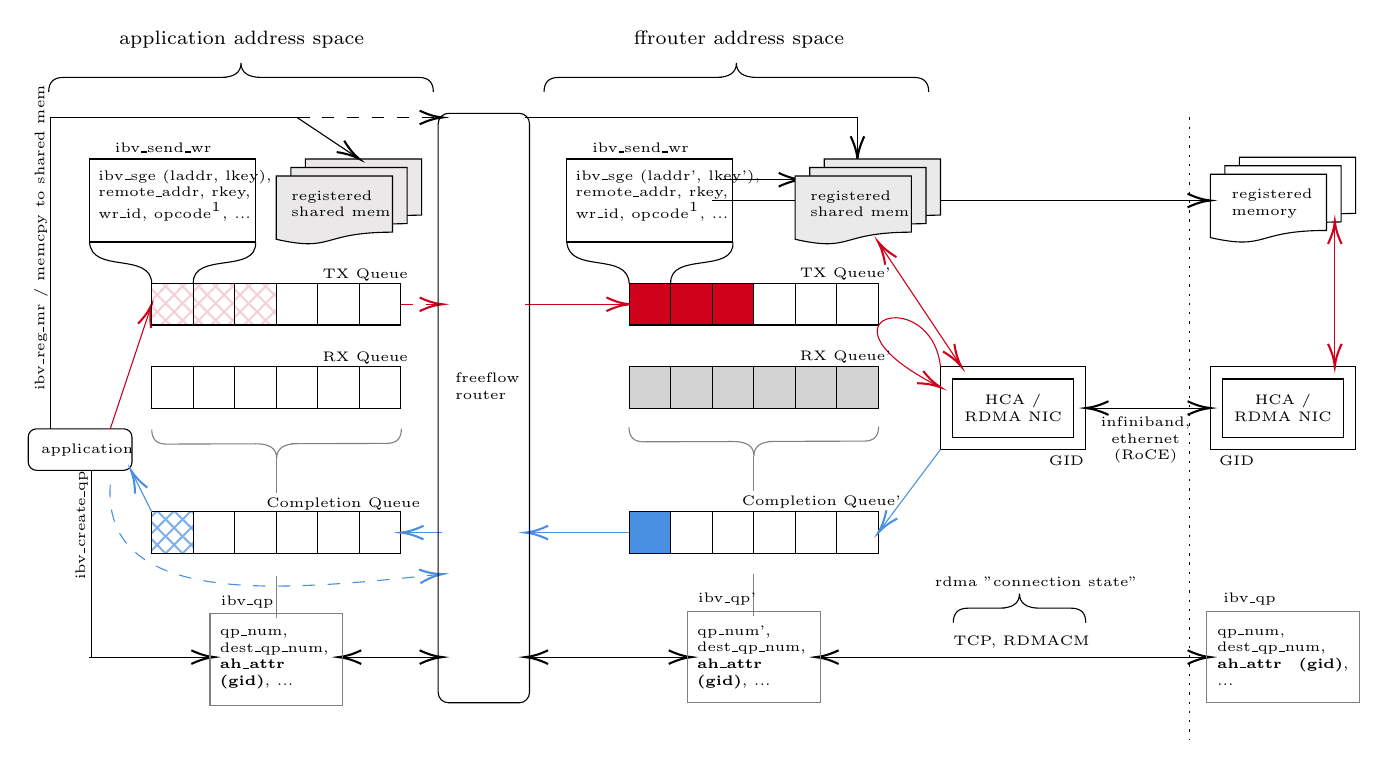
\begin{tikzpicture}[x=0.75pt,y=0.75pt,yscale=-1,xscale=1]
              % Pattern Info

\tikzset{
pattern size/.store in=\mcSize,
pattern size = 5pt,
pattern thickness/.store in=\mcThickness,
pattern thickness = 0.3pt,
pattern radius/.store in=\mcRadius,
pattern radius = 1pt}
\makeatletter
\pgfutil@ifundefined{pgf@pattern@name@_vpzot32ho}{
\pgfdeclarepatternformonly[\mcThickness,\mcSize]{_vpzot32ho}
{\pgfqpoint{0pt}{0pt}}
{\pgfpoint{\mcSize+\mcThickness}{\mcSize+\mcThickness}}
{\pgfpoint{\mcSize}{\mcSize}}
{
\pgfsetcolor{\tikz@pattern@color}
\pgfsetlinewidth{\mcThickness}
\pgfpathmoveto{\pgfqpoint{0pt}{0pt}}
\pgfpathlineto{\pgfpoint{\mcSize+\mcThickness}{\mcSize+\mcThickness}}
\pgfusepath{stroke}
}}
\makeatother

% Pattern Info

\tikzset{
pattern size/.store in=\mcSize,
pattern size = 5pt,
pattern thickness/.store in=\mcThickness,
pattern thickness = 0.3pt,
pattern radius/.store in=\mcRadius,
pattern radius = 1pt}
\makeatletter
\pgfutil@ifundefined{pgf@pattern@name@_mirafmejl}{
\pgfdeclarepatternformonly[\mcThickness,\mcSize]{_mirafmejl}
{\pgfqpoint{0pt}{0pt}}
{\pgfpoint{\mcSize+\mcThickness}{\mcSize+\mcThickness}}
{\pgfpoint{\mcSize}{\mcSize}}
{
\pgfsetcolor{\tikz@pattern@color}
\pgfsetlinewidth{\mcThickness}
\pgfpathmoveto{\pgfqpoint{0pt}{0pt}}
\pgfpathlineto{\pgfpoint{\mcSize+\mcThickness}{\mcSize+\mcThickness}}
\pgfusepath{stroke}
}}
\makeatother

% Pattern Info

\tikzset{
pattern size/.store in=\mcSize,
pattern size = 5pt,
pattern thickness/.store in=\mcThickness,
pattern thickness = 0.3pt,
pattern radius/.store in=\mcRadius,
pattern radius = 1pt}
\makeatletter
\pgfutil@ifundefined{pgf@pattern@name@_d6cbkmj6u}{
\pgfdeclarepatternformonly[\mcThickness,\mcSize]{_d6cbkmj6u}
{\pgfqpoint{0pt}{0pt}}
{\pgfpoint{\mcSize}{\mcSize}}
{\pgfpoint{\mcSize}{\mcSize}}
{
\pgfsetcolor{\tikz@pattern@color}
\pgfsetlinewidth{\mcThickness}
\pgfpathmoveto{\pgfqpoint{0pt}{\mcSize}}
\pgfpathlineto{\pgfpoint{\mcSize+\mcThickness}{-\mcThickness}}
\pgfpathmoveto{\pgfqpoint{0pt}{0pt}}
\pgfpathlineto{\pgfpoint{\mcSize+\mcThickness}{\mcSize+\mcThickness}}
\pgfusepath{stroke}
}}
\makeatother

% Pattern Info

\tikzset{
pattern size/.store in=\mcSize,
pattern size = 5pt,
pattern thickness/.store in=\mcThickness,
pattern thickness = 0.3pt,
pattern radius/.store in=\mcRadius,
pattern radius = 1pt}
\makeatletter
\pgfutil@ifundefined{pgf@pattern@name@_dnbxkzfk8}{
\pgfdeclarepatternformonly[\mcThickness,\mcSize]{_dnbxkzfk8}
{\pgfqpoint{0pt}{0pt}}
{\pgfpoint{\mcSize+\mcThickness}{\mcSize+\mcThickness}}
{\pgfpoint{\mcSize}{\mcSize}}
{
\pgfsetcolor{\tikz@pattern@color}
\pgfsetlinewidth{\mcThickness}
\pgfpathmoveto{\pgfqpoint{0pt}{0pt}}
\pgfpathlineto{\pgfpoint{\mcSize+\mcThickness}{\mcSize+\mcThickness}}
\pgfusepath{stroke}
}}
\makeatother

% Pattern Info

\tikzset{
pattern size/.store in=\mcSize,
pattern size = 5pt,
pattern thickness/.store in=\mcThickness,
pattern thickness = 0.3pt,
pattern radius/.store in=\mcRadius,
pattern radius = 1pt}
\makeatletter
\pgfutil@ifundefined{pgf@pattern@name@_79f3ywchu}{
\pgfdeclarepatternformonly[\mcThickness,\mcSize]{_79f3ywchu}
{\pgfqpoint{0pt}{0pt}}
{\pgfpoint{\mcSize}{\mcSize}}
{\pgfpoint{\mcSize}{\mcSize}}
{
\pgfsetcolor{\tikz@pattern@color}
\pgfsetlinewidth{\mcThickness}
\pgfpathmoveto{\pgfqpoint{0pt}{\mcSize}}
\pgfpathlineto{\pgfpoint{\mcSize+\mcThickness}{-\mcThickness}}
\pgfpathmoveto{\pgfqpoint{0pt}{0pt}}
\pgfpathlineto{\pgfpoint{\mcSize+\mcThickness}{\mcSize+\mcThickness}}
\pgfusepath{stroke}
}}
\makeatother

% Pattern Info

\tikzset{
pattern size/.store in=\mcSize,
pattern size = 5pt,
pattern thickness/.store in=\mcThickness,
pattern thickness = 0.3pt,
pattern radius/.store in=\mcRadius,
pattern radius = 1pt}
\makeatletter
\pgfutil@ifundefined{pgf@pattern@name@_r90kej9lo}{
\pgfdeclarepatternformonly[\mcThickness,\mcSize]{_r90kej9lo}
{\pgfqpoint{0pt}{0pt}}
{\pgfpoint{\mcSize}{\mcSize}}
{\pgfpoint{\mcSize}{\mcSize}}
{
\pgfsetcolor{\tikz@pattern@color}
\pgfsetlinewidth{\mcThickness}
\pgfpathmoveto{\pgfqpoint{0pt}{\mcSize}}
\pgfpathlineto{\pgfpoint{\mcSize+\mcThickness}{-\mcThickness}}
\pgfpathmoveto{\pgfqpoint{0pt}{0pt}}
\pgfpathlineto{\pgfpoint{\mcSize+\mcThickness}{\mcSize+\mcThickness}}
\pgfusepath{stroke}
}}
\makeatother

% Pattern Info

\tikzset{
pattern size/.store in=\mcSize,
pattern size = 5pt,
pattern thickness/.store in=\mcThickness,
pattern thickness = 0.3pt,
pattern radius/.store in=\mcRadius,
pattern radius = 1pt}
\makeatletter
\pgfutil@ifundefined{pgf@pattern@name@_ubeie1m1v}{
\pgfdeclarepatternformonly[\mcThickness,\mcSize]{_ubeie1m1v}
{\pgfqpoint{0pt}{0pt}}
{\pgfpoint{\mcSize}{\mcSize}}
{\pgfpoint{\mcSize}{\mcSize}}
{
\pgfsetcolor{\tikz@pattern@color}
\pgfsetlinewidth{\mcThickness}
\pgfpathmoveto{\pgfqpoint{0pt}{\mcSize}}
\pgfpathlineto{\pgfpoint{\mcSize+\mcThickness}{-\mcThickness}}
\pgfpathmoveto{\pgfqpoint{0pt}{0pt}}
\pgfpathlineto{\pgfpoint{\mcSize+\mcThickness}{\mcSize+\mcThickness}}
\pgfusepath{stroke}
}}
\makeatother
\tikzset{every picture/.style={line width=0.75pt}} %set default line width to 0.75pt

%uncomment if require: \path (0,365); %set diagram left start at 0, and has height of 365

%Shape: Grid [id:dp47924038926915324]
\draw  [draw opacity=0] (330,240) -- (450,240) -- (450,260) -- (330,260) -- cycle ; \draw   (350,240) -- (350,260)(370,240) -- (370,260)(390,240) -- (390,260)(410,240) -- (410,260)(430,240) -- (430,260) ; \draw    ; \draw   (330,240) -- (450,240) -- (450,260) -- (330,260) -- cycle ;
%Shape: Grid [id:dp002167715721618224]
\draw  [draw opacity=0][fill={rgb, 255:red, 210; green, 210; blue, 210 }  ,fill opacity=1 ] (330,170) -- (450,170) -- (450,190) -- (330,190) -- cycle ; \draw   (350,170) -- (350,190)(370,170) -- (370,190)(390,170) -- (390,190)(410,170) -- (410,190)(430,170) -- (430,190) ; \draw    ; \draw   (330,170) -- (450,170) -- (450,190) -- (330,190) -- cycle ;
%Shape: Grid [id:dp7481389991710408]
\draw  [draw opacity=0] (330,130) -- (450,130) -- (450,150) -- (330,150) -- cycle ; \draw   (350,130) -- (350,150)(370,130) -- (370,150)(390,130) -- (390,150)(410,130) -- (410,150)(430,130) -- (430,150) ; \draw    ; \draw   (330,130) -- (450,130) -- (450,150) -- (330,150) -- cycle ;
%Shape: Frame [id:dp12108177355757077]
\draw   (480,170) -- (550,170) -- (550,210) -- (480,210) -- cycle(544,176) -- (486,176) -- (486,204) -- (544,204) -- cycle ;
%Curve Lines [id:da3248928042255319]
\draw [color={rgb, 255:red, 208; green, 2; blue, 27 }  ,draw opacity=1 ]   (480,170) .. controls (475.42,129.8) and (414.41,146.63) .. (479.02,179.5) ;
\draw [shift={(480,180)}, rotate = 206.63] [color={rgb, 255:red, 208; green, 2; blue, 27 }  ,draw opacity=1 ][line width=0.75]    (10.93,-3.29) .. controls (6.95,-1.4) and (3.31,-0.3) .. (0,0) .. controls (3.31,0.3) and (6.95,1.4) .. (10.93,3.29)   ;
%Straight Lines [id:da03676382886970608]
\draw [color={rgb, 255:red, 74; green, 144; blue, 226 }  ,draw opacity=1 ]   (480,210) -- (451.2,248.4) ;
\draw [shift={(450,250)}, rotate = 306.87] [color={rgb, 255:red, 74; green, 144; blue, 226 }  ,draw opacity=1 ][line width=0.75]    (10.93,-3.29) .. controls (6.95,-1.4) and (3.31,-0.3) .. (0,0) .. controls (3.31,0.3) and (6.95,1.4) .. (10.93,3.29)   ;
%Shape: Rectangle [id:dp3450750742562321]
\draw   (300,70) -- (380,70) -- (380,110) -- (300,110) -- cycle ;
%Curve Lines [id:da6906467169425332]
\draw    (330,130) .. controls (329.4,114.4) and (301,125.6) .. (300,110) ;
%Curve Lines [id:da18117978945115543]
\draw    (350,130) .. controls (349.4,114.4) and (381,125.6) .. (380,110) ;
%Shape: Rectangle [id:dp2897498247444361]
\draw  [fill={rgb, 255:red, 208; green, 2; blue, 27 }  ,fill opacity=1 ] (370,130) -- (390,130) -- (390,150) -- (370,150) -- cycle ;
%Shape: Rectangle [id:dp27644727651650536]
\draw  [fill={rgb, 255:red, 208; green, 2; blue, 27 }  ,fill opacity=1 ] (350,130) -- (370,130) -- (370,150) -- (350,150) -- cycle ;
%Shape: Rectangle [id:dp6692701732079035]
\draw  [fill={rgb, 255:red, 208; green, 2; blue, 27 }  ,fill opacity=1 ] (330,130) -- (350,130) -- (350,150) -- (330,150) -- cycle ;
%Shape: Rectangle [id:dp459369140858474]
\draw  [fill={rgb, 255:red, 74; green, 144; blue, 226 }  ,fill opacity=1 ] (330,240) -- (350,240) -- (350,260) -- (330,260) -- cycle ;
%Rounded Rect [id:dp6605095356737472]
\draw   (40.48,204) .. controls (40.48,201.79) and (42.27,200) .. (44.48,200) -- (86.48,200) .. controls (88.69,200) and (90.48,201.79) .. (90.48,204) -- (90.48,216) .. controls (90.48,218.21) and (88.69,220) .. (86.48,220) -- (44.48,220) .. controls (42.27,220) and (40.48,218.21) .. (40.48,216) -- cycle ;
%Straight Lines [id:da34567796721042643]
\draw [color={rgb, 255:red, 208; green, 2; blue, 27 }  ,draw opacity=1 ]   (80,200) -- (99.37,141.9) ;
\draw [shift={(100,140)}, rotate = 468.43] [color={rgb, 255:red, 208; green, 2; blue, 27 }  ,draw opacity=1 ][line width=0.75]    (10.93,-3.29) .. controls (6.95,-1.4) and (3.31,-0.3) .. (0,0) .. controls (3.31,0.3) and (6.95,1.4) .. (10.93,3.29)   ;
%Straight Lines [id:da8473610729667531]
\draw    (375,80) -- (411,80) ;
\draw [shift={(413,80)}, rotate = 180] [color={rgb, 255:red, 0; green, 0; blue, 0 }  ][line width=0.75]    (10.93,-3.29) .. controls (6.95,-1.4) and (3.31,-0.3) .. (0,0) .. controls (3.31,0.3) and (6.95,1.4) .. (10.93,3.29)   ;
%Shape: Frame [id:dp8643269424010532]
\draw   (610,170) -- (680,170) -- (680,210) -- (610,210) -- cycle(674,176) -- (616,176) -- (616,204) -- (674,204) -- cycle ;
%Flowchart: Multidocument [id:dp2723218542370679]
\draw  [fill={rgb, 255:red, 255; green, 255; blue, 255 }  ,fill opacity=1 ] (624,69.17) -- (680,69.17) -- (680,96.23) .. controls (645,96.23) and (652,105.99) .. (624,99.67) -- cycle ; \draw  [fill={rgb, 255:red, 255; green, 255; blue, 255 }  ,fill opacity=1 ] (617,73.27) -- (673,73.27) -- (673,100.33) .. controls (638,100.33) and (645,110.09) .. (617,103.77) -- cycle ; \draw  [fill={rgb, 255:red, 255; green, 255; blue, 255 }  ,fill opacity=1 ] (610,77.37) -- (666,77.37) -- (666,104.43) .. controls (631,104.43) and (638,114.19) .. (610,107.87) -- cycle ;
%Straight Lines [id:da6969742875520862]
\draw [color={rgb, 255:red, 0; green, 0; blue, 0 }  ,draw opacity=1 ]   (552,190) -- (608,190) ;
\draw [shift={(610,190)}, rotate = 180] [color={rgb, 255:red, 0; green, 0; blue, 0 }  ,draw opacity=1 ][line width=0.75]    (10.93,-3.29) .. controls (6.95,-1.4) and (3.31,-0.3) .. (0,0) .. controls (3.31,0.3) and (6.95,1.4) .. (10.93,3.29)   ;
\draw [shift={(550,190)}, rotate = 0] [color={rgb, 255:red, 0; green, 0; blue, 0 }  ,draw opacity=1 ][line width=0.75]    (10.93,-3.29) .. controls (6.95,-1.4) and (3.31,-0.3) .. (0,0) .. controls (3.31,0.3) and (6.95,1.4) .. (10.93,3.29)   ;
%Straight Lines [id:da2204844008555118]
\draw    (422,310) -- (608,310) ;
\draw [shift={(610,310)}, rotate = 180] [color={rgb, 255:red, 0; green, 0; blue, 0 }  ][line width=0.75]    (10.93,-3.29) .. controls (6.95,-1.4) and (3.31,-0.3) .. (0,0) .. controls (3.31,0.3) and (6.95,1.4) .. (10.93,3.29)   ;
\draw [shift={(420,310)}, rotate = 0] [color={rgb, 255:red, 0; green, 0; blue, 0 }  ][line width=0.75]    (10.93,-3.29) .. controls (6.95,-1.4) and (3.31,-0.3) .. (0,0) .. controls (3.31,0.3) and (6.95,1.4) .. (10.93,3.29)   ;
%Shape: Brace [id:dp6301807994328823]
\draw   (550,293.42) .. controls (550,288.75) and (547.67,286.42) .. (543,286.42) -- (528.08,286.42) .. controls (521.41,286.42) and (518.08,284.09) .. (518.08,279.42) .. controls (518.08,284.09) and (514.75,286.42) .. (508.08,286.42)(511.08,286.42) -- (493.17,286.42) .. controls (488.5,286.42) and (486.17,288.75) .. (486.17,293.42) ;
%Straight Lines [id:da4913129650610133]
\draw    (71,220) -- (71,310) ;
%Shape: Brace [id:dp6719984545133558]
\draw  [color={rgb, 255:red, 128; green, 128; blue, 128 }  ,draw opacity=1 ] (329.93,199.28) .. controls (329.95,203.95) and (332.29,206.27) .. (336.96,206.26) -- (380.09,206.13) .. controls (386.76,206.1) and (390.1,208.42) .. (390.11,213.09) .. controls (390.1,208.42) and (393.42,206.08) .. (400.09,206.06)(397.09,206.07) -- (443.22,205.93) .. controls (447.89,205.92) and (450.21,203.58) .. (450.2,198.91) ;
%Straight Lines [id:da042982475702124434]
\draw    (282,310) -- (358,310) ;
\draw [shift={(360,310)}, rotate = 180] [color={rgb, 255:red, 0; green, 0; blue, 0 }  ][line width=0.75]    (10.93,-3.29) .. controls (6.95,-1.4) and (3.31,-0.3) .. (0,0) .. controls (3.31,0.3) and (6.95,1.4) .. (10.93,3.29)   ;
\draw [shift={(280,310)}, rotate = 0] [color={rgb, 255:red, 0; green, 0; blue, 0 }  ][line width=0.75]    (10.93,-3.29) .. controls (6.95,-1.4) and (3.31,-0.3) .. (0,0) .. controls (3.31,0.3) and (6.95,1.4) .. (10.93,3.29)   ;
%Straight Lines [id:da7327906625145184]
\draw [color={rgb, 255:red, 128; green, 128; blue, 128 }  ,draw opacity=1 ]   (390,213) -- (390,230) ;
%Straight Lines [id:da011227227046911814]
\draw [color={rgb, 255:red, 128; green, 128; blue, 128 }  ,draw opacity=1 ]   (390,270) -- (390,290) ;
%Straight Lines [id:da23319890952152877]
\draw    (51,200) -- (51,50) ;
%Straight Lines [id:da7145627673289419]
\draw    (280,50) -- (440,50) ;
%Straight Lines [id:da7243580991907248]
\draw    (440,50) -- (440,68) ;
\draw [shift={(440,70)}, rotate = 270] [color={rgb, 255:red, 0; green, 0; blue, 0 }  ][line width=0.75]    (10.93,-3.29) .. controls (6.95,-1.4) and (3.31,-0.3) .. (0,0) .. controls (3.31,0.3) and (6.95,1.4) .. (10.93,3.29)   ;
%Straight Lines [id:da8759120356182645]
\draw [color={rgb, 255:red, 208; green, 2; blue, 27 }  ,draw opacity=1 ]   (451.11,111.66) -- (488.89,168.34) ;
\draw [shift={(490,170)}, rotate = 236.31] [color={rgb, 255:red, 208; green, 2; blue, 27 }  ,draw opacity=1 ][line width=0.75]    (10.93,-3.29) .. controls (6.95,-1.4) and (3.31,-0.3) .. (0,0) .. controls (3.31,0.3) and (6.95,1.4) .. (10.93,3.29)   ;
\draw [shift={(450,110)}, rotate = 56.31] [color={rgb, 255:red, 208; green, 2; blue, 27 }  ,draw opacity=1 ][line width=0.75]    (10.93,-3.29) .. controls (6.95,-1.4) and (3.31,-0.3) .. (0,0) .. controls (3.31,0.3) and (6.95,1.4) .. (10.93,3.29)   ;
%Straight Lines [id:da1917450897805817]
\draw [color={rgb, 255:red, 208; green, 2; blue, 27 }  ,draw opacity=1 ]   (670,102) -- (670,168) ;
\draw [shift={(670,170)}, rotate = 270] [color={rgb, 255:red, 208; green, 2; blue, 27 }  ,draw opacity=1 ][line width=0.75]    (10.93,-3.29) .. controls (6.95,-1.4) and (3.31,-0.3) .. (0,0) .. controls (3.31,0.3) and (6.95,1.4) .. (10.93,3.29)   ;
\draw [shift={(670,100)}, rotate = 90] [color={rgb, 255:red, 208; green, 2; blue, 27 }  ,draw opacity=1 ][line width=0.75]    (10.93,-3.29) .. controls (6.95,-1.4) and (3.31,-0.3) .. (0,0) .. controls (3.31,0.3) and (6.95,1.4) .. (10.93,3.29)   ;
%Straight Lines [id:da10217296482477001]
\draw    (370,90) -- (608,90) ;
\draw [shift={(610,90)}, rotate = 180] [color={rgb, 255:red, 0; green, 0; blue, 0 }  ][line width=0.75]    (10.93,-3.29) .. controls (6.95,-1.4) and (3.31,-0.3) .. (0,0) .. controls (3.31,0.3) and (6.95,1.4) .. (10.93,3.29)   ;
%Flowchart: Multidocument [id:dp310353723289988]
\draw  [fill={rgb, 255:red, 234; green, 234; blue, 234 }  ,fill opacity=1 ] (424,70) -- (480,70) -- (480,97.06) .. controls (445,97.06) and (452,106.82) .. (424,100.5) -- cycle ; \draw  [fill={rgb, 255:red, 234; green, 234; blue, 234 }  ,fill opacity=1 ] (417,74.1) -- (473,74.1) -- (473,101.16) .. controls (438,101.16) and (445,110.92) .. (417,104.6) -- cycle ; \draw  [fill={rgb, 255:red, 234; green, 234; blue, 234 }  ,fill opacity=1 ] (410,78.2) -- (466,78.2) -- (466,105.26) .. controls (431,105.26) and (438,115.02) .. (410,108.7) -- cycle ;
%Straight Lines [id:da07786460051798183]
\draw  [dash pattern={on 0.84pt off 2.51pt}]  (600,50) -- (600,350) ;
%Shape: Grid [id:dp23690466184986192]
\draw  [draw opacity=0][pattern=_vpzot32ho,pattern size=6pt,pattern thickness=0.75pt,pattern radius=0pt, pattern color={rgb, 255:red, 0; green, 0; blue, 0}] (100,130) -- (220,130) -- (220,150) -- (100,150) -- cycle ; \draw   (120,130) -- (120,150)(140,130) -- (140,150)(160,130) -- (160,150)(180,130) -- (180,150)(200,130) -- (200,150) ; \draw    ; \draw   (100,130) -- (220,130) -- (220,150) -- (100,150) -- cycle ;
%Shape: Grid [id:dp6436108433612562]
\draw  [draw opacity=0][pattern=_mirafmejl,pattern size=6pt,pattern thickness=0.75pt,pattern radius=0pt, pattern color={rgb, 255:red, 210; green, 210; blue, 210}] (100,170) -- (220,170) -- (220,190) -- (100,190) -- cycle ; \draw   (120,170) -- (120,190)(140,170) -- (140,190)(160,170) -- (160,190)(180,170) -- (180,190)(200,170) -- (200,190) ; \draw    ; \draw   (100,170) -- (220,170) -- (220,190) -- (100,190) -- cycle ;
%Shape: Rectangle [id:dp3035895454215348]
\draw  [pattern=_d6cbkmj6u,pattern size=6pt,pattern thickness=0.75pt,pattern radius=0pt, pattern color={rgb, 255:red, 208; green, 2; blue, 27}] (100,130) -- (120,130) -- (120,150) -- (100,150) -- cycle ;
%Straight Lines [id:da8838561898059539]
\draw [color={rgb, 255:red, 208; green, 2; blue, 27 }  ,draw opacity=1 ] [dash pattern={on 4.5pt off 4.5pt}]  (220,140) -- (238,140) ;
\draw [shift={(240,140)}, rotate = 180] [color={rgb, 255:red, 208; green, 2; blue, 27 }  ,draw opacity=1 ][line width=0.75]    (10.93,-3.29) .. controls (6.95,-1.4) and (3.31,-0.3) .. (0,0) .. controls (3.31,0.3) and (6.95,1.4) .. (10.93,3.29)   ;
%Straight Lines [id:da04266110810439505]
\draw [color={rgb, 255:red, 208; green, 2; blue, 27 }  ,draw opacity=1 ]   (280,140) -- (328,140) ;
\draw [shift={(330,140)}, rotate = 180] [color={rgb, 255:red, 208; green, 2; blue, 27 }  ,draw opacity=1 ][line width=0.75]    (10.93,-3.29) .. controls (6.95,-1.4) and (3.31,-0.3) .. (0,0) .. controls (3.31,0.3) and (6.95,1.4) .. (10.93,3.29)   ;
%Shape: Grid [id:dp7998528503897445]
\draw  [draw opacity=0][pattern=_dnbxkzfk8,pattern size=6pt,pattern thickness=0.75pt,pattern radius=0pt, pattern color={rgb, 255:red, 0; green, 0; blue, 0}] (100,240) -- (220,240) -- (220,260) -- (100,260) -- cycle ; \draw   (120,240) -- (120,260)(140,240) -- (140,260)(160,240) -- (160,260)(180,240) -- (180,260)(200,240) -- (200,260) ; \draw    ; \draw   (100,240) -- (220,240) -- (220,260) -- (100,260) -- cycle ;
%Shape: Brace [id:dp4723861809772847]
\draw  [color={rgb, 255:red, 128; green, 128; blue, 128 }  ,draw opacity=1 ] (100,200.38) .. controls (100.01,205.05) and (102.35,207.37) .. (107.02,207.36) -- (150.16,207.22) .. controls (156.83,207.2) and (160.17,209.52) .. (160.18,214.19) .. controls (160.17,209.52) and (163.49,207.18) .. (170.16,207.16)(167.16,207.17) -- (213.29,207.02) .. controls (217.96,207.01) and (220.28,204.67) .. (220.27,200) ;
%Straight Lines [id:da7214579447730238]
\draw [color={rgb, 255:red, 128; green, 128; blue, 128 }  ,draw opacity=1 ]   (160.07,214.09) -- (160.07,231.09) ;
%Straight Lines [id:da7514802764282835]
\draw [color={rgb, 255:red, 128; green, 128; blue, 128 }  ,draw opacity=1 ]   (160.07,271.09) -- (160.07,291.09) ;
%Straight Lines [id:da16494307522388663]
\draw    (70,310) -- (128,310) ;
\draw [shift={(130,310)}, rotate = 180] [color={rgb, 255:red, 0; green, 0; blue, 0 }  ][line width=0.75]    (10.93,-3.29) .. controls (6.95,-1.4) and (3.31,-0.3) .. (0,0) .. controls (3.31,0.3) and (6.95,1.4) .. (10.93,3.29)   ;
%Straight Lines [id:da26029070420114353]
\draw    (192,310) -- (238,310) ;
\draw [shift={(240,310)}, rotate = 180] [color={rgb, 255:red, 0; green, 0; blue, 0 }  ][line width=0.75]    (10.93,-3.29) .. controls (6.95,-1.4) and (3.31,-0.3) .. (0,0) .. controls (3.31,0.3) and (6.95,1.4) .. (10.93,3.29)   ;
\draw [shift={(190,310)}, rotate = 0] [color={rgb, 255:red, 0; green, 0; blue, 0 }  ][line width=0.75]    (10.93,-3.29) .. controls (6.95,-1.4) and (3.31,-0.3) .. (0,0) .. controls (3.31,0.3) and (6.95,1.4) .. (10.93,3.29)   ;
%Straight Lines [id:da5537140126718904]
\draw    (51,50) -- (170,50) ;
%Straight Lines [id:da016019539589035015]
\draw [color={rgb, 255:red, 74; green, 144; blue, 226 }  ,draw opacity=1 ]   (240,250) -- (222,250) ;
\draw [shift={(220,250)}, rotate = 360] [color={rgb, 255:red, 74; green, 144; blue, 226 }  ,draw opacity=1 ][line width=0.75]    (10.93,-3.29) .. controls (6.95,-1.4) and (3.31,-0.3) .. (0,0) .. controls (3.31,0.3) and (6.95,1.4) .. (10.93,3.29)   ;
%Straight Lines [id:da9940166448903683]
\draw [color={rgb, 255:red, 74; green, 144; blue, 226 }  ,draw opacity=1 ]   (330,250) -- (282,250) ;
\draw [shift={(280,250)}, rotate = 360] [color={rgb, 255:red, 74; green, 144; blue, 226 }  ,draw opacity=1 ][line width=0.75]    (10.93,-3.29) .. controls (6.95,-1.4) and (3.31,-0.3) .. (0,0) .. controls (3.31,0.3) and (6.95,1.4) .. (10.93,3.29)   ;
%Curve Lines [id:da11215835101687177]
\draw [color={rgb, 255:red, 74; green, 144; blue, 226 }  ,draw opacity=1 ] [dash pattern={on 4.5pt off 4.5pt}]  (80,227) .. controls (76.02,288.19) and (168.73,277.28) .. (238.94,270.11) ;
\draw [shift={(240,270)}, rotate = 534.1800000000001] [color={rgb, 255:red, 74; green, 144; blue, 226 }  ,draw opacity=1 ][line width=0.75]    (10.93,-3.29) .. controls (6.95,-1.4) and (3.31,-0.3) .. (0,0) .. controls (3.31,0.3) and (6.95,1.4) .. (10.93,3.29)   ;
%Shape: Rectangle [id:dp5705528003005959]
\draw  [pattern=_79f3ywchu,pattern size=6pt,pattern thickness=0.75pt,pattern radius=0pt, pattern color={rgb, 255:red, 74; green, 144; blue, 226}] (100,240) -- (120,240) -- (120,260) -- (100,260) -- cycle ;
%Shape: Rectangle [id:dp5643123604055056]
\draw   (70,70) -- (150,70) -- (150,110) -- (70,110) -- cycle ;
%Curve Lines [id:da2381444493403747]
\draw    (100,130) .. controls (99.4,114.4) and (71,125.6) .. (70,110) ;
%Curve Lines [id:da0014333330861757698]
\draw    (120,130) .. controls (119.4,114.4) and (151,125.6) .. (150,110) ;
%Flowchart: Multidocument [id:dp4127879431820818]
\draw  [fill={rgb, 255:red, 234; green, 232; blue, 232 }  ,fill opacity=1 ] (174,70) -- (230,70) -- (230,97.06) .. controls (195,97.06) and (202,106.82) .. (174,100.5) -- cycle ; \draw  [fill={rgb, 255:red, 234; green, 232; blue, 232 }  ,fill opacity=1 ] (167,74.1) -- (223,74.1) -- (223,101.16) .. controls (188,101.16) and (195,110.92) .. (167,104.6) -- cycle ; \draw  [fill={rgb, 255:red, 234; green, 232; blue, 232 }  ,fill opacity=1 ] (160,78.2) -- (216,78.2) -- (216,105.26) .. controls (181,105.26) and (188,115.02) .. (160,108.7) -- cycle ;
%Shape: Brace [id:dp780601608855469]
\draw  [color={rgb, 255:red, 0; green, 0; blue, 0 }  ,draw opacity=1 ] (235.67,37.71) .. controls (235.67,33.04) and (233.34,30.71) .. (228.67,30.71) -- (153,30.71) .. controls (146.33,30.71) and (143,28.38) .. (143,23.71) .. controls (143,28.38) and (139.67,30.71) .. (133,30.71)(136,30.71) -- (57.33,30.71) .. controls (52.66,30.71) and (50.33,33.04) .. (50.33,37.71) ;
%Shape: Brace [id:dp6850978046359238]
\draw  [color={rgb, 255:red, 0; green, 0; blue, 0 }  ,draw opacity=1 ] (474.33,37.71) .. controls (474.33,33.04) and (472,30.71) .. (467.33,30.71) -- (391.67,30.71) .. controls (385,30.71) and (381.67,28.38) .. (381.67,23.71) .. controls (381.67,28.38) and (378.34,30.71) .. (371.67,30.71)(374.67,30.71) -- (296,30.71) .. controls (291.33,30.71) and (289,33.04) .. (289,37.71) ;
%Straight Lines [id:da029343615050499317]
\draw    (170,50) -- (198.34,68.89) ;
\draw [shift={(200,70)}, rotate = 213.69] [color={rgb, 255:red, 0; green, 0; blue, 0 }  ][line width=0.75]    (10.93,-3.29) .. controls (6.95,-1.4) and (3.31,-0.3) .. (0,0) .. controls (3.31,0.3) and (6.95,1.4) .. (10.93,3.29)   ;
%Straight Lines [id:da9471146626002113]
\draw  [dash pattern={on 4.5pt off 4.5pt}]  (170,50) -- (238,50) ;
\draw [shift={(240,50)}, rotate = 180] [color={rgb, 255:red, 0; green, 0; blue, 0 }  ][line width=0.75]    (10.93,-3.29) .. controls (6.95,-1.4) and (3.31,-0.3) .. (0,0) .. controls (3.31,0.3) and (6.95,1.4) .. (10.93,3.29)   ;
%Shape: Rectangle [id:dp13305705707797522]
\draw  [pattern=_r90kej9lo,pattern size=6pt,pattern thickness=0.75pt,pattern radius=0pt, pattern color={rgb, 255:red, 208; green, 2; blue, 27}] (120,130) -- (140,130) -- (140,150) -- (120,150) -- cycle ;
%Shape: Rectangle [id:dp2317469012582416]
\draw  [pattern=_ubeie1m1v,pattern size=6pt,pattern thickness=0.75pt,pattern radius=0pt, pattern color={rgb, 255:red, 208; green, 2; blue, 27}] (140,130) -- (160,130) -- (160,150) -- (140,150) -- cycle ;
%Straight Lines [id:da22053909576707187]
\draw [color={rgb, 255:red, 74; green, 144; blue, 226 }  ,draw opacity=1 ]   (100,240) -- (90.89,221.79) ;
\draw [shift={(90,220)}, rotate = 423.43] [color={rgb, 255:red, 74; green, 144; blue, 226 }  ,draw opacity=1 ][line width=0.75]    (10.93,-3.29) .. controls (6.95,-1.4) and (3.31,-0.3) .. (0,0) .. controls (3.31,0.3) and (6.95,1.4) .. (10.93,3.29)   ;

% Text Node
\draw (383,231) node [anchor=north west][inner sep=0.75pt]  [font=\tiny] [align=left] {Completion Queue'};
% Text Node
\draw (411,121) node [anchor=north west][inner sep=0.75pt]  [font=\tiny] [align=left] {TX Queue'};
% Text Node
\draw (411,161) node [anchor=north west][inner sep=0.75pt]  [font=\tiny] [align=left] {RX Queue'};
% Text Node
\draw (311,61) node [anchor=north west][inner sep=0.75pt]  [font=\tiny] [align=left] {ibv\_send\_wr};
% Text Node
\draw (303,74) node [anchor=north west][inner sep=0.75pt]  [font=\tiny] [align=left] {ibv\_sge (laddr', lkey'),\\remote\_addr, rkey,\\wr\_id, opcode$\displaystyle ^{1}$, ...};
% Text Node
\draw (45.48,206) node [anchor=north west][inner sep=0.75pt]  [font=\tiny] [align=left] {application};
% Text Node
\draw (416,84) node [anchor=north west][inner sep=0.75pt]  [font=\tiny] [align=left] {registered\\shared mem};
% Text Node
\draw (42,183) node [anchor=north west][inner sep=0.75pt]  [font=\tiny,rotate=-270] [align=left] {ibv\_reg\_mr / memcpy to shared mem};
% Text Node
\draw (619,83.17) node [anchor=north west][inner sep=0.75pt]  [font=\tiny] [align=left] {registered\\memory};
% Text Node
\draw (551,193) node [anchor=north west][inner sep=0.75pt]  [font=\tiny] [align=left] {\begin{minipage}[lt]{39.83664400000001pt}\setlength\topsep{0pt}
\begin{center}
infiniband,\\ethernet (RoCE)
\end{center}

\end{minipage}};
% Text Node
\draw (515,190) node  [font=\tiny] [align=left] {\begin{minipage}[lt]{39.440000000000005pt}\setlength\topsep{0pt}
\begin{center}
HCA /\\RDMA NIC
\end{center}

\end{minipage}};
% Text Node
\draw (645,190) node  [font=\tiny] [align=left] {\begin{minipage}[lt]{39.440000000000005pt}\setlength\topsep{0pt}
\begin{center}
HCA /\\RDMA NIC
\end{center}

\end{minipage}};
% Text Node
\draw (531,212) node [anchor=north west][inner sep=0.75pt]  [font=\tiny] [align=left] {GID};
% Text Node
\draw (613,212) node [anchor=north west][inner sep=0.75pt]  [font=\tiny] [align=left] {GID};
% Text Node
\draw  [color={rgb, 255:red, 128; green, 128; blue, 128 }  ,draw opacity=1 ]  (358,288) -- (422,288) -- (422,332) -- (358,332) -- cycle  ;
\draw (390,310) node  [font=\tiny] [align=left] {\begin{minipage}[lt]{40.800000000000004pt}\setlength\topsep{0pt}
qp\_num', dest\_qp\_num, \textbf{ah\_attr (gid)}, ...
\end{minipage}};
% Text Node
\draw (362,278) node [anchor=north west][inner sep=0.75pt]  [font=\tiny] [align=left] {ibv\_qp'};
% Text Node
\draw (476,270) node [anchor=north west][inner sep=0.75pt]  [font=\tiny] [align=left] {rdma "connection state"};
% Text Node
\draw (62,274) node [anchor=north west][inner sep=0.75pt]  [font=\tiny,rotate=-270] [align=left] {ibv\_create\_qp};
% Text Node
\draw (519,303) node  [font=\tiny] [align=left] {\begin{minipage}[lt]{68pt}\setlength\topsep{0pt}
\begin{center}
TCP, RDMACM
\end{center}

\end{minipage}};
% Text Node
\draw  [color={rgb, 255:red, 128; green, 128; blue, 128 }  ,draw opacity=1 ]  (608,288) -- (682,288) -- (682,332) -- (608,332) -- cycle  ;
\draw (645,310) node  [font=\tiny] [align=left] {\begin{minipage}[lt]{47.6pt}\setlength\topsep{0pt}
qp\_num, dest\_qp\_num, \textbf{ah\_attr (gid)}, ...
\end{minipage}};
% Text Node
\draw (615,278) node [anchor=north west][inner sep=0.75pt]  [font=\tiny] [align=left] {ibv\_qp};
% Text Node
\draw    (238,53) .. controls (238,50.24) and (240.24,48) .. (243,48) -- (277,48) .. controls (279.76,48) and (282,50.24) .. (282,53) -- (282,327) .. controls (282,329.76) and (279.76,332) .. (277,332) -- (243,332) .. controls (240.24,332) and (238,329.76) .. (238,327) -- cycle  ;
\draw (260,190) node  [font=\tiny] [align=left] {\begin{minipage}[lt]{27.200000000000003pt}\setlength\topsep{0pt}
\begin{center}
\end{center}

\end{minipage}};
% Text Node
\draw (181,122) node [anchor=north west][inner sep=0.75pt]  [font=\tiny] [align=left] {TX Queue};
% Text Node
\draw (181,162) node [anchor=north west][inner sep=0.75pt]  [font=\tiny] [align=left] {RX Queue};
% Text Node
\draw (245,172) node [anchor=north west][inner sep=0.75pt]  [font=\tiny] [align=left] {freeflow\\router};
% Text Node
\draw (154,232) node [anchor=north west][inner sep=0.75pt]  [font=\tiny] [align=left] {Completion Queue};
% Text Node
\draw  [color={rgb, 255:red, 128; green, 128; blue, 128 }  ,draw opacity=1 ]  (128.07,289.09) -- (192.07,289.09) -- (192.07,333.09) -- (128.07,333.09) -- cycle  ;
\draw (160.07,311.09) node  [font=\tiny] [align=left] {\begin{minipage}[lt]{40.800000000000004pt}\setlength\topsep{0pt}
qp\_num, dest\_qp\_num, \textbf{ah\_attr (gid)}, ...
\end{minipage}};
% Text Node
\draw (132.07,279.09) node [anchor=north west][inner sep=0.75pt]  [font=\tiny] [align=left] {ibv\_qp};
% Text Node
\draw (81,61) node [anchor=north west][inner sep=0.75pt]  [font=\tiny] [align=left] {ibv\_send\_wr};
% Text Node
\draw (73,74) node [anchor=north west][inner sep=0.75pt]  [font=\tiny] [align=left] {ibv\_sge (laddr, lkey),\\remote\_addr, rkey,\\wr\_id, opcode$\displaystyle ^{1}$, ...};
% Text Node
\draw (166,84) node [anchor=north west][inner sep=0.75pt]  [font=\tiny] [align=left] {registered\\shared mem};
% Text Node
\draw (83,7) node [anchor=north west][inner sep=0.75pt]  [font=\scriptsize] [align=left] {application address space};
% Text Node
\draw (331,7) node [anchor=north west][inner sep=0.75pt]  [font=\scriptsize] [align=left] {ffrouter address space};

          \end{tikzpicture}
      }
    \column{.40\textwidth}
        \includegraphics[width=0.9\textwidth]{freeflowrdmasend.png}
        \vspace{-10pt}
        \begin{center}
            \fontsize{4pt}{4pt}\selectfont source: FreeFlow Paper Figure 5
        \end{center}
    \end{columns}
\end{frame}

\begin{frame}{FreeFlow Library --- Router Communication}
    \begin{itemize}
        \item IPC communication
            \begin{itemize}
                \item Latency can be $\geq 5\mu s$
            \end{itemize}
        \item Fastpath
            \begin{itemize}
                \item Move \texttt{TX Queue} and \texttt{RX Queue} to shared memory with FreeFlow router
                \item FreeFlow router spin reads these queue pairs (with cache flushes)
            \end{itemize}
    \end{itemize}
\end{frame}

\begin{frame}{FreeFlow Challenges \& Solutions}
    \begin{itemize}
        \item Use shared memory to support and speed up one-sided operations.
            \begin{itemize}
                \item Requires \texttt{malloc} highjack to page align memory.
                \item New functions \texttt{ibv\_malloc} and \texttt{ibv\_free} to avoid this.
                \item ffrouter must replace \texttt{laddr} with \texttt{laddr'}
            \end{itemize}
        \item Utilize \texttt{libibverb}'s built in struct flattening to avoid deep copies in RPC.
        \item Multiple Unix sockets for parallel RDMA queue pairs to avoid head of line blocking.
    \end{itemize}
\end{frame}

\begin{frame}{FreeFlow Benefits}
    \begin{itemize}
        \item Control plane policy enforcement on queue pairs.
            \begin{itemize}
                \item QoS and network overlay enforcements
            \end{itemize}
        \item RDMA vNIC can be assigned a private IP, allowing for non-live container migration.
            \begin{itemize}
                \item ffrouter can query network overlays to get private IP -$>$ public IP translation.
            \end{itemize}
        \item FreeFlow library can run TCP over RDMA using \texttt{rsocket} in \texttt{libibverbs}.
    \end{itemize}
\end{frame}

\begin{frame}{FreeFlow Performance}
    \begin{figure}
        \centering
        \begin{minipage}{.45\textwidth}
        \includegraphics[width=\textwidth]{perfgraph1.png}
        \vspace{-25pt}
        \begin{center}
            \fontsize{4pt}{4pt}\selectfont source: FreeFlow Paper Figure 9
        \end{center}

        \end{minipage}%
        \hspace{10pt}%
        \begin{minipage}{.45\textwidth}
        \includegraphics[width=\textwidth]{perfgraph2.png}
        \vspace{-25pt}
        \begin{center}
            \fontsize{4pt}{4pt}\selectfont source: FreeFlow Paper Figure 10
        \end{center}
        \end{minipage}
        \begin{minipage}{.25\textwidth}
        \includegraphics[width=\textwidth]{perfgraph3.png}
        \vspace{-25pt}
        \begin{center}
            \fontsize{4pt}{4pt}\selectfont source: FreeFlow Paper Figure 12
        \end{center}
        \end{minipage}
    \end{figure}

    \begin{itemize}
        \item Approx 33\% increase in latency for small messages
        \item Small message sizes bound in tput due to Fastpath single thread bottleneck
        \item Non-Fastpath CPU util overhead scales with actual load
            \begin{itemize}
                \item Fastpath requires at least a single CPU core
            \end{itemize}
        \item Applications finish at close to host RDMA speeds
    \end{itemize}
\end{frame}

\section{Hardware Approach}

\begin{frame}{SRIOV}
    \begin{center}
        \includegraphics[width=0.6\textwidth]{sriovmlnx.png}
    \end{center}

    \begin{itemize}
        \item Not portable.
        \item Control plane policy enforcement relies on switch reconfiguration.
    \end{itemize}
\end{frame}

\begin{frame}{MACVLAN}
    \begin{center}
        \includegraphics[width=0.6\textwidth]{macvlanmnlx.png}
    \end{center}

    \begin{itemize}
        \item Control plane policy enforcement relies on switch reconfiguration?
        \item ``GID table entries are created whenever an IP address is configured on one of the Ethernet devices of the NIC's ports.''
    \end{itemize}
\end{frame}

\begin{frame}{RDMA Shared Device}
    \begin{itemize}
        \item RDMA namespaces
        \item RDMA cgroups
        \item ConnectX6 NICs allow for hardware rules?
    \end{itemize}
\end{frame}

% \section{Discussion}
% \begin{frame}
%     \begin{itemize}
%         \item Why is Microsoft and Mellanox pushing for hardware-based isolation when FreeFlow appears to provide these isolations with minimum overhead?
%         \item Can FreeFlow sufficiently express existing container network policy?
%         \item Could FreeFlow be applied to other kernel bypass networking solutions?
%         \item Is this better than zero-copy networking with the standard kernel TCP stack?
%     \end{itemize}
% \end{frame}


\end{document}
